\documentclass[11pt]{article}

% Shared notes settings for Applied Machine Learning lectures (UPES).
% Keep this file free of \documentclass to allow reuse via \input.

\usepackage[utf8]{inputenc}
\usepackage[T1]{fontenc}
\usepackage{lmodern}          % scalable T1 fonts; without this pdflatex falls back
\input{glyphtounicode}        % to bitmapped EC Type 3 and the PDFs are neither
\pdfgentounicode=1            % searchable nor screen-reader friendly
\usepackage[a4paper,margin=1in]{geometry}
\usepackage{hyperref}
\usepackage{xurl}
\usepackage{booktabs}
\usepackage{amsmath}
\usepackage{amssymb}
\usepackage{listings}
\usepackage{xcolor}
\usepackage{enumitem}
\usepackage{parskip}

% Code listings (Python-oriented for this subject).
\lstset{
  language=Python,
  basicstyle=\ttfamily\small,
  keywordstyle=\color{blue},
  commentstyle=\color{gray},
  stringstyle=\color{teal},
  showstringspaces=false,
  columns=fullflexible,
  frame=single,
  framerule=0.2pt,
  breaklines=true
}

\setlist[itemize]{topsep=0.3em,itemsep=0.2em}
\setlist[enumerate]{topsep=0.3em,itemsep=0.2em}

% Simple per-section source line.
\newcommand{\notesources}[1]{\par\noindent{\small\color{gray}\textit{Sources:} \sloppy #1\par}}

% Unit-wise source strings for this subject (used by slides + notes).
% Path is relative to the lecture `latex/` folder (the compilation CWD).
\IfFileExists{../../../_shared/aml-sources.tex}{%
  % Source strings for Applied Machine Learning (CSAI2017P) — used by slides + notes.
% Prescribed texts and reference books are taken from the course syllabus.
% Support texts are the author-hosted open-access editions:
%   statlearning.com            (ISL with Python)
%   probml.github.io/pml-book   (Murphy, Probabilistic Machine Learning)
%   d2l.ai                      (Dive into Deep Learning)
%   mml-book.github.io          (Mathematics for Machine Learning)

\newcommand{\AMLRepoURL}{https://github.com/tali7c/Applied-Machine-Learning}

% --- prescribed -------------------------------------------------------------
\newcommand{\AMLPrescribed}{%
M\"uller and Guido, \textit{Introduction to Machine Learning with Python}, O'Reilly, 2016.;%
Bishop, \textit{Pattern Recognition and Machine Learning}, Springer, 2006.;%
Murphy, \textit{Machine Learning: A Probabilistic Perspective}, MIT Press, 2012.;%
Han, Kamber and Pei, \textit{Data Mining: Concepts and Techniques} (3e), Morgan Kaufmann, 2012.%
}

% --- unit-wise ---------------------------------------------------------------
\newcommand{\AMLUnitISources}{%
M\"uller and Guido, \textit{Introduction to Machine Learning with Python}, Ch. 1.;%
Bishop, \textit{Pattern Recognition and Machine Learning}, Ch. 1.;%
Murphy, \textit{Probabilistic Machine Learning: An Introduction}, MIT Press, 2022, Ch. 1.;%
Mitchell, \textit{Machine Learning}, McGraw Hill, 1997, Ch. 1.;%
Scikit-learn documentation, accessed 2026-08-04.%
}

\newcommand{\AMLUnitIISources}{%
Bishop, \textit{Pattern Recognition and Machine Learning}, \S1.5, \S4.3, \S7.1.;%
Zhang, Lipton, Li and Smola, \textit{Dive into Deep Learning}, \S3.4.;%
Shalev-Shwartz and Ben-David, \textit{Understanding Machine Learning}, Ch. 15.;%
Murphy, \textit{Probabilistic Machine Learning: An Introduction}, Ch. 5.%
}

\newcommand{\AMLUnitIIISources}{%
Zhang, Lipton, Li and Smola, \textit{Dive into Deep Learning}, Ch. 12 (Optimization Algorithms).;%
Deisenroth, Faisal and Ong, \textit{Mathematics for Machine Learning}, Ch. 7.;%
Kingma and Ba, ``Adam: A Method for Stochastic Optimization,'' ICLR 2015.;%
Ruder, ``An overview of gradient descent optimization algorithms,'' arXiv:1609.04747, 2016.%
}

\newcommand{\AMLUnitIVSources}{%
Han, Kamber and Pei, \textit{Data Mining: Concepts and Techniques} (3e), Ch. 3.;%
M\"uller and Guido, \textit{Introduction to Machine Learning with Python}, Ch. 3--4.;%
James, Witten, Hastie, Tibshirani and Taylor, \textit{An Introduction to Statistical Learning with Python}, Ch. 5--6, 12.;%
Scikit-learn documentation (preprocessing, model selection), accessed 2026-08-04.%
}

\newcommand{\AMLUnitVSources}{%
James et al., \textit{An Introduction to Statistical Learning with Python}, Ch. 3--6.;%
Bishop, \textit{Pattern Recognition and Machine Learning}, Ch. 3.;%
Deisenroth, Faisal and Ong, \textit{Mathematics for Machine Learning}, Ch. 9.;%
M\"uller and Guido, \textit{Introduction to Machine Learning with Python}, \S2.3.%
}

\newcommand{\AMLUnitVISources}{%
Han, Kamber and Pei, \textit{Data Mining: Concepts and Techniques} (3e), Ch. 8--9.;%
James et al., \textit{An Introduction to Statistical Learning with Python}, Ch. 8--9.;%
Bishop, \textit{Pattern Recognition and Machine Learning}, Ch. 4--5, 7, 14.;%
Zhang et al., \textit{Dive into Deep Learning}, Ch. 5.%
}

\newcommand{\AMLUnitVIISources}{%
Han, Kamber and Pei, \textit{Data Mining: Concepts and Techniques} (3e), Ch. 10.;%
James et al., \textit{An Introduction to Statistical Learning with Python}, Ch. 12.;%
M\"uller and Guido, \textit{Introduction to Machine Learning with Python}, \S3.5.;%
Ester, Kriegel, Sander and Xu, ``A density-based algorithm for discovering clusters (DBSCAN),'' KDD 1996.%
}

\newcommand{\AMLLabSources}{%
M\"uller and Guido, \textit{Introduction to Machine Learning with Python}, companion notebooks.;%
McKinney, \textit{Python for Data Analysis} (3e), O'Reilly, 2022.;%
Scikit-learn user guide, accessed 2026-08-04.;%
Matplotlib and Seaborn documentation, accessed 2026-08-04.%
}
%
}{%
  % Faculty copies live under `private/` so their compile CWD is different.
  \IfFileExists{../../../../public/_shared/aml-sources.tex}{%
    % Source strings for Applied Machine Learning (CSAI2017P) — used by slides + notes.
% Prescribed texts and reference books are taken from the course syllabus.
% Support texts are the author-hosted open-access editions:
%   statlearning.com            (ISL with Python)
%   probml.github.io/pml-book   (Murphy, Probabilistic Machine Learning)
%   d2l.ai                      (Dive into Deep Learning)
%   mml-book.github.io          (Mathematics for Machine Learning)

\newcommand{\AMLRepoURL}{https://github.com/tali7c/Applied-Machine-Learning}

% --- prescribed -------------------------------------------------------------
\newcommand{\AMLPrescribed}{%
M\"uller and Guido, \textit{Introduction to Machine Learning with Python}, O'Reilly, 2016.;%
Bishop, \textit{Pattern Recognition and Machine Learning}, Springer, 2006.;%
Murphy, \textit{Machine Learning: A Probabilistic Perspective}, MIT Press, 2012.;%
Han, Kamber and Pei, \textit{Data Mining: Concepts and Techniques} (3e), Morgan Kaufmann, 2012.%
}

% --- unit-wise ---------------------------------------------------------------
\newcommand{\AMLUnitISources}{%
M\"uller and Guido, \textit{Introduction to Machine Learning with Python}, Ch. 1.;%
Bishop, \textit{Pattern Recognition and Machine Learning}, Ch. 1.;%
Murphy, \textit{Probabilistic Machine Learning: An Introduction}, MIT Press, 2022, Ch. 1.;%
Mitchell, \textit{Machine Learning}, McGraw Hill, 1997, Ch. 1.;%
Scikit-learn documentation, accessed 2026-08-04.%
}

\newcommand{\AMLUnitIISources}{%
Bishop, \textit{Pattern Recognition and Machine Learning}, \S1.5, \S4.3, \S7.1.;%
Zhang, Lipton, Li and Smola, \textit{Dive into Deep Learning}, \S3.4.;%
Shalev-Shwartz and Ben-David, \textit{Understanding Machine Learning}, Ch. 15.;%
Murphy, \textit{Probabilistic Machine Learning: An Introduction}, Ch. 5.%
}

\newcommand{\AMLUnitIIISources}{%
Zhang, Lipton, Li and Smola, \textit{Dive into Deep Learning}, Ch. 12 (Optimization Algorithms).;%
Deisenroth, Faisal and Ong, \textit{Mathematics for Machine Learning}, Ch. 7.;%
Kingma and Ba, ``Adam: A Method for Stochastic Optimization,'' ICLR 2015.;%
Ruder, ``An overview of gradient descent optimization algorithms,'' arXiv:1609.04747, 2016.%
}

\newcommand{\AMLUnitIVSources}{%
Han, Kamber and Pei, \textit{Data Mining: Concepts and Techniques} (3e), Ch. 3.;%
M\"uller and Guido, \textit{Introduction to Machine Learning with Python}, Ch. 3--4.;%
James, Witten, Hastie, Tibshirani and Taylor, \textit{An Introduction to Statistical Learning with Python}, Ch. 5--6, 12.;%
Scikit-learn documentation (preprocessing, model selection), accessed 2026-08-04.%
}

\newcommand{\AMLUnitVSources}{%
James et al., \textit{An Introduction to Statistical Learning with Python}, Ch. 3--6.;%
Bishop, \textit{Pattern Recognition and Machine Learning}, Ch. 3.;%
Deisenroth, Faisal and Ong, \textit{Mathematics for Machine Learning}, Ch. 9.;%
M\"uller and Guido, \textit{Introduction to Machine Learning with Python}, \S2.3.%
}

\newcommand{\AMLUnitVISources}{%
Han, Kamber and Pei, \textit{Data Mining: Concepts and Techniques} (3e), Ch. 8--9.;%
James et al., \textit{An Introduction to Statistical Learning with Python}, Ch. 8--9.;%
Bishop, \textit{Pattern Recognition and Machine Learning}, Ch. 4--5, 7, 14.;%
Zhang et al., \textit{Dive into Deep Learning}, Ch. 5.%
}

\newcommand{\AMLUnitVIISources}{%
Han, Kamber and Pei, \textit{Data Mining: Concepts and Techniques} (3e), Ch. 10.;%
James et al., \textit{An Introduction to Statistical Learning with Python}, Ch. 12.;%
M\"uller and Guido, \textit{Introduction to Machine Learning with Python}, \S3.5.;%
Ester, Kriegel, Sander and Xu, ``A density-based algorithm for discovering clusters (DBSCAN),'' KDD 1996.%
}

\newcommand{\AMLLabSources}{%
M\"uller and Guido, \textit{Introduction to Machine Learning with Python}, companion notebooks.;%
McKinney, \textit{Python for Data Analysis} (3e), O'Reilly, 2022.;%
Scikit-learn user guide, accessed 2026-08-04.;%
Matplotlib and Seaborn documentation, accessed 2026-08-04.%
}
%
  }{%
    % Question papers live at `private/<family>/<instrument>/`.
    \IfFileExists{../../../public/_shared/aml-sources.tex}{%
      % Source strings for Applied Machine Learning (CSAI2017P) — used by slides + notes.
% Prescribed texts and reference books are taken from the course syllabus.
% Support texts are the author-hosted open-access editions:
%   statlearning.com            (ISL with Python)
%   probml.github.io/pml-book   (Murphy, Probabilistic Machine Learning)
%   d2l.ai                      (Dive into Deep Learning)
%   mml-book.github.io          (Mathematics for Machine Learning)

\newcommand{\AMLRepoURL}{https://github.com/tali7c/Applied-Machine-Learning}

% --- prescribed -------------------------------------------------------------
\newcommand{\AMLPrescribed}{%
M\"uller and Guido, \textit{Introduction to Machine Learning with Python}, O'Reilly, 2016.;%
Bishop, \textit{Pattern Recognition and Machine Learning}, Springer, 2006.;%
Murphy, \textit{Machine Learning: A Probabilistic Perspective}, MIT Press, 2012.;%
Han, Kamber and Pei, \textit{Data Mining: Concepts and Techniques} (3e), Morgan Kaufmann, 2012.%
}

% --- unit-wise ---------------------------------------------------------------
\newcommand{\AMLUnitISources}{%
M\"uller and Guido, \textit{Introduction to Machine Learning with Python}, Ch. 1.;%
Bishop, \textit{Pattern Recognition and Machine Learning}, Ch. 1.;%
Murphy, \textit{Probabilistic Machine Learning: An Introduction}, MIT Press, 2022, Ch. 1.;%
Mitchell, \textit{Machine Learning}, McGraw Hill, 1997, Ch. 1.;%
Scikit-learn documentation, accessed 2026-08-04.%
}

\newcommand{\AMLUnitIISources}{%
Bishop, \textit{Pattern Recognition and Machine Learning}, \S1.5, \S4.3, \S7.1.;%
Zhang, Lipton, Li and Smola, \textit{Dive into Deep Learning}, \S3.4.;%
Shalev-Shwartz and Ben-David, \textit{Understanding Machine Learning}, Ch. 15.;%
Murphy, \textit{Probabilistic Machine Learning: An Introduction}, Ch. 5.%
}

\newcommand{\AMLUnitIIISources}{%
Zhang, Lipton, Li and Smola, \textit{Dive into Deep Learning}, Ch. 12 (Optimization Algorithms).;%
Deisenroth, Faisal and Ong, \textit{Mathematics for Machine Learning}, Ch. 7.;%
Kingma and Ba, ``Adam: A Method for Stochastic Optimization,'' ICLR 2015.;%
Ruder, ``An overview of gradient descent optimization algorithms,'' arXiv:1609.04747, 2016.%
}

\newcommand{\AMLUnitIVSources}{%
Han, Kamber and Pei, \textit{Data Mining: Concepts and Techniques} (3e), Ch. 3.;%
M\"uller and Guido, \textit{Introduction to Machine Learning with Python}, Ch. 3--4.;%
James, Witten, Hastie, Tibshirani and Taylor, \textit{An Introduction to Statistical Learning with Python}, Ch. 5--6, 12.;%
Scikit-learn documentation (preprocessing, model selection), accessed 2026-08-04.%
}

\newcommand{\AMLUnitVSources}{%
James et al., \textit{An Introduction to Statistical Learning with Python}, Ch. 3--6.;%
Bishop, \textit{Pattern Recognition and Machine Learning}, Ch. 3.;%
Deisenroth, Faisal and Ong, \textit{Mathematics for Machine Learning}, Ch. 9.;%
M\"uller and Guido, \textit{Introduction to Machine Learning with Python}, \S2.3.%
}

\newcommand{\AMLUnitVISources}{%
Han, Kamber and Pei, \textit{Data Mining: Concepts and Techniques} (3e), Ch. 8--9.;%
James et al., \textit{An Introduction to Statistical Learning with Python}, Ch. 8--9.;%
Bishop, \textit{Pattern Recognition and Machine Learning}, Ch. 4--5, 7, 14.;%
Zhang et al., \textit{Dive into Deep Learning}, Ch. 5.%
}

\newcommand{\AMLUnitVIISources}{%
Han, Kamber and Pei, \textit{Data Mining: Concepts and Techniques} (3e), Ch. 10.;%
James et al., \textit{An Introduction to Statistical Learning with Python}, Ch. 12.;%
M\"uller and Guido, \textit{Introduction to Machine Learning with Python}, \S3.5.;%
Ester, Kriegel, Sander and Xu, ``A density-based algorithm for discovering clusters (DBSCAN),'' KDD 1996.%
}

\newcommand{\AMLLabSources}{%
M\"uller and Guido, \textit{Introduction to Machine Learning with Python}, companion notebooks.;%
McKinney, \textit{Python for Data Analysis} (3e), O'Reilly, 2022.;%
Scikit-learn user guide, accessed 2026-08-04.;%
Matplotlib and Seaborn documentation, accessed 2026-08-04.%
}
%
    }{%
      % Marking schemes live at `private/solutions/<family>/<id>/latex/`.
      \IfFileExists{../../../../../public/_shared/aml-sources.tex}{%
        % Source strings for Applied Machine Learning (CSAI2017P) — used by slides + notes.
% Prescribed texts and reference books are taken from the course syllabus.
% Support texts are the author-hosted open-access editions:
%   statlearning.com            (ISL with Python)
%   probml.github.io/pml-book   (Murphy, Probabilistic Machine Learning)
%   d2l.ai                      (Dive into Deep Learning)
%   mml-book.github.io          (Mathematics for Machine Learning)

\newcommand{\AMLRepoURL}{https://github.com/tali7c/Applied-Machine-Learning}

% --- prescribed -------------------------------------------------------------
\newcommand{\AMLPrescribed}{%
M\"uller and Guido, \textit{Introduction to Machine Learning with Python}, O'Reilly, 2016.;%
Bishop, \textit{Pattern Recognition and Machine Learning}, Springer, 2006.;%
Murphy, \textit{Machine Learning: A Probabilistic Perspective}, MIT Press, 2012.;%
Han, Kamber and Pei, \textit{Data Mining: Concepts and Techniques} (3e), Morgan Kaufmann, 2012.%
}

% --- unit-wise ---------------------------------------------------------------
\newcommand{\AMLUnitISources}{%
M\"uller and Guido, \textit{Introduction to Machine Learning with Python}, Ch. 1.;%
Bishop, \textit{Pattern Recognition and Machine Learning}, Ch. 1.;%
Murphy, \textit{Probabilistic Machine Learning: An Introduction}, MIT Press, 2022, Ch. 1.;%
Mitchell, \textit{Machine Learning}, McGraw Hill, 1997, Ch. 1.;%
Scikit-learn documentation, accessed 2026-08-04.%
}

\newcommand{\AMLUnitIISources}{%
Bishop, \textit{Pattern Recognition and Machine Learning}, \S1.5, \S4.3, \S7.1.;%
Zhang, Lipton, Li and Smola, \textit{Dive into Deep Learning}, \S3.4.;%
Shalev-Shwartz and Ben-David, \textit{Understanding Machine Learning}, Ch. 15.;%
Murphy, \textit{Probabilistic Machine Learning: An Introduction}, Ch. 5.%
}

\newcommand{\AMLUnitIIISources}{%
Zhang, Lipton, Li and Smola, \textit{Dive into Deep Learning}, Ch. 12 (Optimization Algorithms).;%
Deisenroth, Faisal and Ong, \textit{Mathematics for Machine Learning}, Ch. 7.;%
Kingma and Ba, ``Adam: A Method for Stochastic Optimization,'' ICLR 2015.;%
Ruder, ``An overview of gradient descent optimization algorithms,'' arXiv:1609.04747, 2016.%
}

\newcommand{\AMLUnitIVSources}{%
Han, Kamber and Pei, \textit{Data Mining: Concepts and Techniques} (3e), Ch. 3.;%
M\"uller and Guido, \textit{Introduction to Machine Learning with Python}, Ch. 3--4.;%
James, Witten, Hastie, Tibshirani and Taylor, \textit{An Introduction to Statistical Learning with Python}, Ch. 5--6, 12.;%
Scikit-learn documentation (preprocessing, model selection), accessed 2026-08-04.%
}

\newcommand{\AMLUnitVSources}{%
James et al., \textit{An Introduction to Statistical Learning with Python}, Ch. 3--6.;%
Bishop, \textit{Pattern Recognition and Machine Learning}, Ch. 3.;%
Deisenroth, Faisal and Ong, \textit{Mathematics for Machine Learning}, Ch. 9.;%
M\"uller and Guido, \textit{Introduction to Machine Learning with Python}, \S2.3.%
}

\newcommand{\AMLUnitVISources}{%
Han, Kamber and Pei, \textit{Data Mining: Concepts and Techniques} (3e), Ch. 8--9.;%
James et al., \textit{An Introduction to Statistical Learning with Python}, Ch. 8--9.;%
Bishop, \textit{Pattern Recognition and Machine Learning}, Ch. 4--5, 7, 14.;%
Zhang et al., \textit{Dive into Deep Learning}, Ch. 5.%
}

\newcommand{\AMLUnitVIISources}{%
Han, Kamber and Pei, \textit{Data Mining: Concepts and Techniques} (3e), Ch. 10.;%
James et al., \textit{An Introduction to Statistical Learning with Python}, Ch. 12.;%
M\"uller and Guido, \textit{Introduction to Machine Learning with Python}, \S3.5.;%
Ester, Kriegel, Sander and Xu, ``A density-based algorithm for discovering clusters (DBSCAN),'' KDD 1996.%
}

\newcommand{\AMLLabSources}{%
M\"uller and Guido, \textit{Introduction to Machine Learning with Python}, companion notebooks.;%
McKinney, \textit{Python for Data Analysis} (3e), O'Reilly, 2022.;%
Scikit-learn user guide, accessed 2026-08-04.;%
Matplotlib and Seaborn documentation, accessed 2026-08-04.%
}
%
      }{%
        % Source strings for Applied Machine Learning (CSAI2017P) — used by slides + notes.
% Prescribed texts and reference books are taken from the course syllabus.
% Support texts are the author-hosted open-access editions:
%   statlearning.com            (ISL with Python)
%   probml.github.io/pml-book   (Murphy, Probabilistic Machine Learning)
%   d2l.ai                      (Dive into Deep Learning)
%   mml-book.github.io          (Mathematics for Machine Learning)

\newcommand{\AMLRepoURL}{https://github.com/tali7c/Applied-Machine-Learning}

% --- prescribed -------------------------------------------------------------
\newcommand{\AMLPrescribed}{%
M\"uller and Guido, \textit{Introduction to Machine Learning with Python}, O'Reilly, 2016.;%
Bishop, \textit{Pattern Recognition and Machine Learning}, Springer, 2006.;%
Murphy, \textit{Machine Learning: A Probabilistic Perspective}, MIT Press, 2012.;%
Han, Kamber and Pei, \textit{Data Mining: Concepts and Techniques} (3e), Morgan Kaufmann, 2012.%
}

% --- unit-wise ---------------------------------------------------------------
\newcommand{\AMLUnitISources}{%
M\"uller and Guido, \textit{Introduction to Machine Learning with Python}, Ch. 1.;%
Bishop, \textit{Pattern Recognition and Machine Learning}, Ch. 1.;%
Murphy, \textit{Probabilistic Machine Learning: An Introduction}, MIT Press, 2022, Ch. 1.;%
Mitchell, \textit{Machine Learning}, McGraw Hill, 1997, Ch. 1.;%
Scikit-learn documentation, accessed 2026-08-04.%
}

\newcommand{\AMLUnitIISources}{%
Bishop, \textit{Pattern Recognition and Machine Learning}, \S1.5, \S4.3, \S7.1.;%
Zhang, Lipton, Li and Smola, \textit{Dive into Deep Learning}, \S3.4.;%
Shalev-Shwartz and Ben-David, \textit{Understanding Machine Learning}, Ch. 15.;%
Murphy, \textit{Probabilistic Machine Learning: An Introduction}, Ch. 5.%
}

\newcommand{\AMLUnitIIISources}{%
Zhang, Lipton, Li and Smola, \textit{Dive into Deep Learning}, Ch. 12 (Optimization Algorithms).;%
Deisenroth, Faisal and Ong, \textit{Mathematics for Machine Learning}, Ch. 7.;%
Kingma and Ba, ``Adam: A Method for Stochastic Optimization,'' ICLR 2015.;%
Ruder, ``An overview of gradient descent optimization algorithms,'' arXiv:1609.04747, 2016.%
}

\newcommand{\AMLUnitIVSources}{%
Han, Kamber and Pei, \textit{Data Mining: Concepts and Techniques} (3e), Ch. 3.;%
M\"uller and Guido, \textit{Introduction to Machine Learning with Python}, Ch. 3--4.;%
James, Witten, Hastie, Tibshirani and Taylor, \textit{An Introduction to Statistical Learning with Python}, Ch. 5--6, 12.;%
Scikit-learn documentation (preprocessing, model selection), accessed 2026-08-04.%
}

\newcommand{\AMLUnitVSources}{%
James et al., \textit{An Introduction to Statistical Learning with Python}, Ch. 3--6.;%
Bishop, \textit{Pattern Recognition and Machine Learning}, Ch. 3.;%
Deisenroth, Faisal and Ong, \textit{Mathematics for Machine Learning}, Ch. 9.;%
M\"uller and Guido, \textit{Introduction to Machine Learning with Python}, \S2.3.%
}

\newcommand{\AMLUnitVISources}{%
Han, Kamber and Pei, \textit{Data Mining: Concepts and Techniques} (3e), Ch. 8--9.;%
James et al., \textit{An Introduction to Statistical Learning with Python}, Ch. 8--9.;%
Bishop, \textit{Pattern Recognition and Machine Learning}, Ch. 4--5, 7, 14.;%
Zhang et al., \textit{Dive into Deep Learning}, Ch. 5.%
}

\newcommand{\AMLUnitVIISources}{%
Han, Kamber and Pei, \textit{Data Mining: Concepts and Techniques} (3e), Ch. 10.;%
James et al., \textit{An Introduction to Statistical Learning with Python}, Ch. 12.;%
M\"uller and Guido, \textit{Introduction to Machine Learning with Python}, \S3.5.;%
Ester, Kriegel, Sander and Xu, ``A density-based algorithm for discovering clusters (DBSCAN),'' KDD 1996.%
}

\newcommand{\AMLLabSources}{%
M\"uller and Guido, \textit{Introduction to Machine Learning with Python}, companion notebooks.;%
McKinney, \textit{Python for Data Analysis} (3e), O'Reilly, 2022.;%
Scikit-learn user guide, accessed 2026-08-04.;%
Matplotlib and Seaborn documentation, accessed 2026-08-04.%
}
%
      }%
    }%
  }%
}


\graphicspath{{../figures/}}

% This lecture pairs almost every paragraph with a listing and its output, so
% the default \medskipamount around each block adds up to several pages.
\lstset{aboveskip=2pt, belowskip=2pt}
% `parskip` sets ~0.5\baselineskip between paragraphs; with this many short
% paragraphs interleaved with code that alone is worth two pages.
\setlength{\parskip}{0.32\baselineskip plus 1.5pt}
% Local override of the shared `amlout` style: this lecture pairs almost
% every paragraph with an output block, so the shared 8pt belowskip adds up.
\lstdefinestyle{amlout}{
  language={}, keepspaces=true,
  basicstyle=\ttfamily\footnotesize\color{black!80},
  backgroundcolor=\color{black!4},
  frame=leftline, framerule=2pt, rulecolor=\color{black!25},
  breaklines=true, columns=fullflexible, xleftmargin=8pt,
  aboveskip=1pt, belowskip=4pt, literate={-}{{-}}1
}
\captionsetup{skip=4pt, font=small}
% Eleven wide figures in a text-dense document: let them share pages with
% prose instead of being pushed onto float pages of their own.
\renewcommand{\topfraction}{0.92}
\renewcommand{\bottomfraction}{0.75}
\renewcommand{\textfraction}{0.06}
\renewcommand{\floatpagefraction}{0.85}
\setlength{\floatsep}{6pt plus 2pt minus 2pt}
\setlength{\textfloatsep}{8pt plus 2pt minus 2pt}
\setlength{\intextsep}{8pt plus 2pt minus 2pt}

\title{Applied Machine Learning\\Unit 07 --- Lecture 21 Notes\\
       Similarity Measures and Data Types in Clustering}
\author{Tofik Ali}
\date{Autumn 2026}

\begin{document}
\maketitle

\begin{keyidea}[Read this first]
These notes are written so that you can learn the material \emph{without}
having been in the lecture. Every concept is developed from scratch, every
number you see was produced by running the code shown beside it, and every
figure was generated from real computation rather than drawn by hand.

The previous lecture said that clustering groups objects so that objects in
the same group are \emph{similar} and objects in different groups are not,
and then left the word ``similar'' undefined. Every algorithm in this unit
--- hierarchical clustering, $k$-means, $k$-medoids, DBSCAN --- takes a
\textbf{distance} as its input. Not the data: the distances. Change the
distance and you change the answer, without touching a line of the
algorithm.

This lecture is about getting that distance right before running anything.
Three numbers carry it and you should be able to reproduce all three with a
pen. First, Section~\ref{sec:binary}: three patients, six binary tests,
$q=2$, $r=0$, $s=1$, $t=3$, simple matching $0.8333$ against Jaccard
$0.6667$ --- and a pair of examples where the two coefficients rank
\emph{the same two pairs in opposite orders}. Second,
Section~\ref{sec:mixed}: four applicants with numeric, ordinal, nominal and
asymmetric binary attributes, $d(A,B) = \mathbf{0.340686}$ with every
$\delta_f$ written out. Third, Section~\ref{sec:centroid}: two three-point
clusters, single $5.000000$, centroid $5.656854$, average $5.715413$,
complete $6.403124$. Those three calculations are the examinable arithmetic
of this lecture, and the assessment that follows it will ask for them.
\end{keyidea}

\tableofcontents
\medskip

% =========================================================================
\section{How to use these notes}
\label{sec:how}

Read in order. Sections~\ref{sec:vocab} to \ref{sec:cosine} are one
continuous argument about numeric attributes; Sections~\ref{sec:binary} to
\ref{sec:mixed} do the harder and more examinable half, what to do when the
columns are not numbers at all; Section~\ref{sec:standard} is the warning
that applies to everything before it; and Section~\ref{sec:centroid} sets up
the hierarchical clustering of the next lecture. Everything here assumes the
$k$-nearest-neighbour lecture, where feature scaling first appeared --- there
it changed a classifier's accuracy, here it changes which object is nearest,
and those are the same fact.

There are four kinds of box. \textbf{Key idea} --- the one sentence to
remember a month from now. \textbf{Worked example} --- a calculation done by
hand, with small numbers, before any library is used. \textbf{Caution} ---
the specific mistake that section exists to prevent. \textbf{Try it
yourself} --- something to run, with the expected output given so you can
check.

Code appears in a framed block, and directly beneath it a shaded block
showing what that code \emph{actually printed}. If you run it and get
something different, trust your machine and tell me.

\subsection{What you need}

\begin{lstlisting}
pip install numpy scipy scikit-learn matplotlib
\end{lstlisting}

Every number in these notes was produced with:

\begin{lstlisting}
import numpy, scipy, sklearn, matplotlib
print("numpy", numpy.__version__, "| scipy", scipy.__version__,
      "| sklearn", sklearn.__version__,
      "| matplotlib", matplotlib.__version__)
\end{lstlisting}
\begin{codeout}
numpy 2.2.6 | scipy 1.15.3 | sklearn 1.7.2 | matplotlib 3.10.9
\end{codeout}

Three bundled datasets recur, and \textbf{none of them downloads anything}:

\begin{lstlisting}
from sklearn.datasets import load_iris, load_wine, load_breast_cancer
\end{lstlisting}
\begin{codeout}
load_iris           150 rows x  4 features, 3 classes
load_wine           178 rows x 13 features, 3 classes
load_breast_cancer  569 rows x 30 features, 2 classes
no download: every loader above reads a CSV inside the package
wine feature scales differ by three orders of magnitude:
  alcohol          min    11.030  max    14.830  sd     0.810
  magnesium        min    70.000  max   162.000  sd    14.242
  proline          min   278.000  max  1680.000  sd   314.022
\end{codeout}

Everything else is a small table constructed inline in the code, small enough
that you can check it with a pen. That is deliberate: this is a lecture about
arithmetic you should be able to do yourself.

\begin{caution}[Do not reach for \texttt{fetch\_*}]
Every \texttt{fetch\_*} loader downloads over HTTPS, and on the campus network
those downloads fail with a certificate error you cannot fix from your machine.
Nothing in this course depends on one: use the bundled loaders or a small
table you build yourself.
\end{caution}

\begin{keyidea}[One seed, and only three places it is used]
Almost nothing in this lecture is random: the tables are written out by hand
and the datasets are bundled. Where a random draw \emph{is} needed --- the
$200$ points that check the metric axioms, the $400$ pairs that check the
Minkowski ordering, and the one \texttt{KMeans} fit in the closing comparison
--- there is \textbf{one seed, $0$}, written as
\texttt{np.random.default\_rng(0)} or \texttt{random\_state=0}, and every
listing shows it rather than hiding it in a helper.

So every number printed in these notes reproduces \emph{exactly} if you run
the code as written. If yours differs, the difference is in your code or your
library versions, not in chance --- which is the only thing that makes a
printed number worth anything to you.
\end{keyidea}

\subsection{Learning outcomes}

These notes serve \textbf{CO1} --- \emph{understand the fundamental concepts,
terminology and mathematical foundations of machine learning} --- and
\textbf{CO2} --- \emph{apply appropriate machine learning techniques and
demonstrate the underlying computation}. By the end you should be able to:

\begin{enumerate}[leftmargin=*]
  \item Distinguish a similarity from a dissimilarity, convert between them,
    and state what the dissimilarity matrix is and why it, rather than the
    data, is what a clustering algorithm consumes. \hfill \textbf{CO1}
  \item State the four metric axioms and \textbf{name a measure that violates
    each}, with a numerical counter-example. \hfill \textbf{CO1}
  \item Compute Manhattan, Euclidean, Minkowski-$p$ and Chebyshev distances
    by hand for a given pair, and explain what $p$ controls. \hfill
    \textbf{CO2}
  \item Compute cosine similarity by hand, state exactly what it discards,
    and give a pair on which it and Euclidean distance disagree. \hfill
    \textbf{CO2}
  \item Build the $2\times2$ contingency table for two binary objects and
    compute the simple matching and Jaccard coefficients, choosing correctly
    between them on the symmetric/asymmetric distinction. \hfill \textbf{CO2}
  \item Compute the nominal mismatch ratio $(p-m)/p$, and say precisely when
    one-hot encoding reproduces it and when it does not. \hfill \textbf{CO2}
  \item Map an ordinal attribute with $(r-1)/(M-1)$ and state the assumption
    that map makes. \hfill \textbf{CO1}
  \item Compute a Gower dissimilarity across mixed attribute types by hand,
    including the $\delta_f = 0$ rule for asymmetric binary attributes.
    \hfill \textbf{CO2}
  \item Explain and demonstrate that standardisation changes which object is
    nearest, and contrast z-score with mean-absolute-deviation scaling.
    \hfill \textbf{CO1, CO2}
  \item Compute a cluster centroid and medoid, and the single, complete,
    average and centroid distances between two clusters. \hfill \textbf{CO2}
\end{enumerate}

% =========================================================================
\section{Similarity, dissimilarity, and the object the algorithm eats}
\label{sec:vocab}

Two words are used throughout this unit and they are not interchangeable.

A \textbf{similarity} $s(i,j)$ is large when objects $i$ and $j$ are alike.
It is usually scaled so that $s \in [0,1]$ and $s(i,i) = 1$. Cosine
similarity, the Jaccard coefficient and the simple matching coefficient are
all similarities.

A \textbf{dissimilarity} $d(i,j)$ is small when the objects are alike, with
$d(i,i) = 0$. Euclidean distance is a dissimilarity. So is $1 - s$ for any
similarity living in $[0,1]$.

You can convert between them freely --- $d = 1-s$, or $d = \sqrt{2(1-s)}$, or
$s = 1/(1+d)$ --- but you should convert \emph{deliberately}, because the
conversion changes the geometry. Section~\ref{sec:cosine} contains a case
where $1-s$ is not a metric but $\sqrt{2(1-s)}$ is.

\begin{keyidea}[The dissimilarity matrix is the interface]
A clustering algorithm does not consume your data table. It consumes the
$n \times n$ \textbf{dissimilarity matrix} $D$, with $D_{ij} = d(i,j)$,
symmetric with a zero diagonal. Everything you decide in this lecture --- the
metric, the treatment of each column type, the scaling --- is decided
\emph{before} $D$ is built. After that the algorithm is just a rule for
grouping the entries of a table of numbers, and it cannot recover information
you threw away when you built it.
\end{keyidea}

That matrix is also what you pay for. It has $n(n-1)/2$ distinct entries:

\begin{lstlisting}
from scipy.spatial.distance import pdist, squareform
Xi = StandardScaler().fit_transform(load_iris().data)
Di = pdist(Xi, "euclidean")
\end{lstlisting}
\begin{codeout}
iris: 150 objects -> 11175 pairwise distances, n(n-1)/2
condensed 11175 floats = 87.3 KB;  square 150 x 150 = 175.8 KB
         n              pairs  MB at 8 bytes
       150              11175            0.1
      1000             499500            4.0
     10000           49995000          400.0
    100000         4999950000        39999.6
\end{codeout}

At a hundred thousand objects the dissimilarity matrix alone is forty
gigabytes. This is why the hierarchical methods of the next lecture are
quadratic in memory and why $k$-means, which never forms the matrix, scales
further. Note also \texttt{scipy}'s \emph{condensed} form: it stores only the
upper triangle, which is half the memory of the square form, and
\texttt{squareform} converts between the two.

% =========================================================================
\section{What a distance has to be: the metric axioms}
\label{sec:axioms}

A dissimilarity $d$ is a \textbf{metric} if it satisfies four conditions for
all objects $i$, $j$, $k$:

\begin{align}
  &\text{non-negativity} & d(i,j) &\ge 0 \label{eq:ax1}\\
  &\text{identity of indiscernibles} & d(i,j) &= 0 \iff i = j \label{eq:ax2}\\
  &\text{symmetry} & d(i,j) &= d(j,i) \label{eq:ax3}\\
  &\text{triangle inequality} & d(i,k) &\le d(i,j) + d(j,k) \label{eq:ax4}
\end{align}

These are not decoration. Axiom~\eqref{eq:ax3} is what makes ``the distance
between $i$ and $j$'' a well-defined phrase at all, and without it a
clustering could depend on the order in which you read the rows.
Axiom~\eqref{eq:ax4} says no detour is shorter than the direct route, and
that is what licenses every algorithmic shortcut in the neighbour-search
literature: $k$-d trees, ball trees, and the triangle-inequality pruning that
makes Elkan's $k$-means fast all use it to skip comparisons they can prove
are unnecessary. Feed such an implementation a measure that violates
\eqref{eq:ax4} and it will return a wrong answer without complaining.

Euclidean distance satisfies all four. Here is the check, on two hundred
random points in $\mathbb{R}^4$:

\begin{lstlisting}
import itertools, numpy as np
from scipy.spatial.distance import pdist, squareform
rng = np.random.default_rng(0)
D = squareform(pdist(rng.normal(size=(200, 4)), "euclidean"))
off = ~np.eye(200, dtype=bool)
print(D[off].min(), np.abs(np.diag(D)).max(), np.abs(D - D.T).max())
worst = max(D[i, k] - (D[i, j] + D[j, k])
            for i, j, k in itertools.combinations(range(60), 3))
\end{lstlisting}
\begin{codeout}
non-negativity   min off-diagonal d = 0.169507  (>= 0)
identity         max |d(i,i)|        = 0.000000  (== 0)
identity         any d(i,j)==0 for i!=j : False
symmetry         max |d(i,j)-d(j,i)| = 0.000e+00
triangle         max d(i,k)-(d(i,j)+d(j,k)) = -0.007349  (<= 0)
\end{codeout}

The triangle line is the interesting one. Over the $\binom{60}{3} = 34\,220$
triples the \emph{worst} slack is $-0.007349$: the inequality is never
violated, but it comes close, which is exactly what you would expect from a
nearly collinear triple.

\subsection{Three named measures that fail}
\label{sec:violators}

The axioms only earn their place if you can name something that breaks them.

\begin{worked}[Squared Euclidean distance fails the triangle inequality]
Three points on a line: $a = (0,0)$, $b = (1,0)$, $c = (2,0)$. Write
$d^2(u,v) = \sum_f (u_f - v_f)^2$, with no square root.
\[
  d^2(a,b) = 1, \qquad d^2(b,c) = 1, \qquad d^2(a,c) = 4
\]
\[
  d^2(a,c) = 4 \;>\; 1 + 1 = d^2(a,b) + d^2(b,c)
\]
Axiom~\eqref{eq:ax4} fails. \ensuremath{\square}
\end{worked}

\begin{lstlisting}
d2 = lambda u, v: float(np.sum((u - v)**2))
a, b, c = np.array([0., 0.]), np.array([1., 0.]), np.array([2., 0.])
\end{lstlisting}
\begin{codeout}
a=(0,0)  b=(1,0)  c=(2,0)
d2(a,b) = 1.0000   d2(b,c) = 1.0000   sum = 2.0000
d2(a,c) = 4.0000   -> 4.0000 > 2.0000, triangle inequality FAILS
(this is what k-means minimises; it is a divergence, not a metric)
\end{codeout}

This is not an exotic case. Squared Euclidean distance is precisely what
$k$-means minimises, which is why $k$-means is described as minimising a
\emph{divergence} rather than a distance, and why the triangle-inequality
guarantees available to hierarchical clustering are not available to it.
Squaring is a monotone transformation, so the \emph{ranking} of pairs is
unchanged --- what breaks is the arithmetic \emph{between} distances, and
that is what \eqref{eq:ax4} is about.

The second violator is more surprising because it is one of the two measures
this lecture spends most time on.

\begin{worked}[Cosine distance fails the triangle inequality]
Let $\mathrm{cd}(x,y) = 1 - \cos(x,y)$. Take $A = (1,0)$, $B = (1,1)$,
$C = (0,1)$. The angle $A$ to $B$ is $45^\circ$, $B$ to $C$ is $45^\circ$,
and $A$ to $C$ is $90^\circ$.
\[
  \mathrm{cd}(A,B) = 1 - \tfrac{1}{\sqrt2} = 0.292893, \qquad
  \mathrm{cd}(B,C) = 0.292893, \qquad
  \mathrm{cd}(A,C) = 1 - 0 = 1
\]
\[
  0.292893 + 0.292893 = 0.585786 \;<\; 1
\]
The detour through $B$ is \emph{cheaper} than going straight from $A$ to $C$.
\ensuremath{\square}
\end{worked}

\begin{codeout}
cd(A,B) = 0.292893   cd(B,C) = 0.292893   sum = 0.585786
cd(A,C) = 1.000000   -> 1.000000 > 0.585786, triangle inequality FAILS
angular distance arccos(cos)/pi repairs it:
  0.250000 + 0.250000 = 0.500000  >=  0.500000  OK
\end{codeout}

The repair is to use the \textbf{angular distance}
$\arccos(\cos\theta)/\pi$, which is proportional to the angle itself rather
than to one minus its cosine. On the same three vectors it gives
$0.25 + 0.25 = 0.5$ exactly, so the inequality holds with equality --- which
is right, because $B$ really does lie on the shortest arc from $A$ to $C$.
The other repair, used constantly in practice, is $\sqrt{2(1-\cos)}$; we
derive it in Section~\ref{sec:cosine} and it turns out to be Euclidean
distance on normalised vectors, hence a metric.

\begin{figure}[htbp]
  \centering
  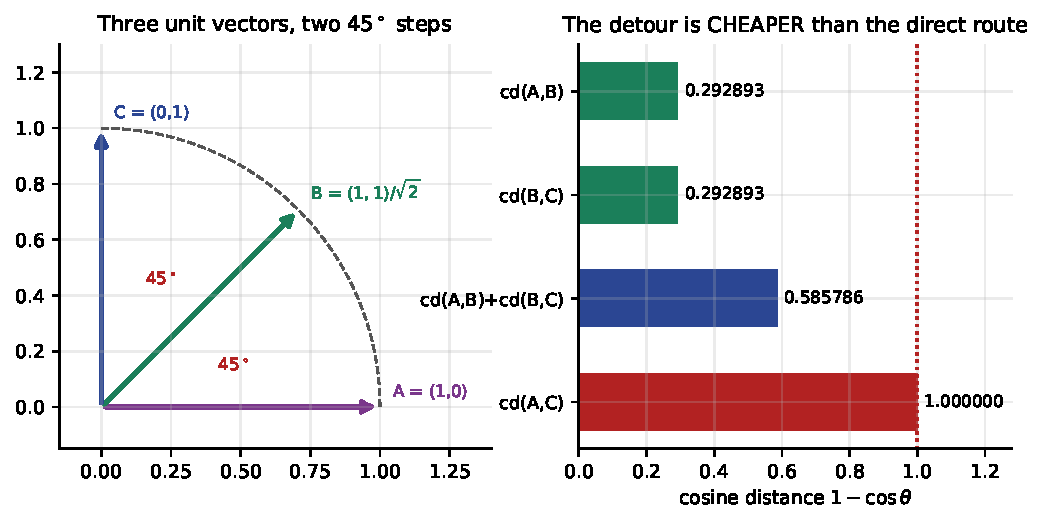
\includegraphics[width=0.78\textwidth]{triangle_violation.pdf}
  \caption{Cosine distance violating the triangle inequality. Left: three
    unit vectors, two $45^\circ$ steps and one $90^\circ$ step. Right: the
    sum of the two short hops, $0.585786$, is smaller than the direct
    distance, $1.000000$.}
  \label{fig:triangle}
\end{figure}

The third violator fails a different axiom.

\begin{lstlisting}
kl = lambda u, v: float(np.sum(u * np.log2(u / v)))
p, q = np.array([0.5, 0.3, 0.2]), np.array([0.2, 0.4, 0.4])
print(kl(p, q), kl(q, p))
\end{lstlisting}
\begin{codeout}
p = [0.5 0.3 0.2]   q = [0.2 0.4 0.4]
KL(p||q) = 0.336453   KL(q||p) = 0.301629   difference 0.034823
symmetry FAILS, so 'the distance between p and q' is not defined
until you say which way round -- and clustering needs it defined.
\end{codeout}

The Kullback--Leibler divergence between two probability distributions is not
symmetric: $\mathrm{KL}(p\|q) \ne \mathrm{KL}(q\|p)$. It is a perfectly good
tool --- it is the loss that trains almost every classifier you have met ---
but it is not a distance, and ``the KL distance between two clusters'' is not
a well-formed phrase. The symmetrised version
$\tfrac12\big(\mathrm{KL}(p\|q) + \mathrm{KL}(q\|p)\big)$ repairs
\eqref{eq:ax3} but still fails \eqref{eq:ax4}; the Jensen--Shannon
\emph{distance}, the square root of the Jensen--Shannon divergence, is a
genuine metric.

Here is the summary table for everything this lecture uses:

\begin{codeout}
measure                  d>=0  d(i,i)=0  symmetry  triangle
Euclidean                 yes       yes       yes       yes
Manhattan                 yes       yes       yes       yes
Minkowski p>=1            yes       yes       yes       yes
Chebyshev                 yes       yes       yes       yes
squared Euclidean         yes       yes       yes        NO
cosine distance           yes       no*       yes        NO
Jaccard distance          yes       yes       yes       yes
simple matching dist      yes       yes       yes       yes
KL divergence             yes       yes        NO        NO
* cosine distance is 0 for any two PARALLEL vectors, not only for
  equal ones: cd((1,2),(2,4)) = 0.000000
\end{codeout}

Read the asterisk carefully, because it is the half of \eqref{eq:ax2} that
people forget. $d(i,i) = 0$ is easy; the hard direction is
$d(i,j) = 0 \Rightarrow i = j$. Cosine distance fails it: $(1,2)$ and
$(2,4)$ are different objects at distance zero. In clustering terms, cosine
declares two objects identical whenever they differ only in magnitude ---
which, as Section~\ref{sec:cosine} argues, is sometimes exactly what you
want.

% =========================================================================
\section{Numeric attributes: the Minkowski family}
\label{sec:minkowski}

Almost every distance you will use on numeric attributes is one member of a
single family with one dial:

\begin{equation}
  d_p(x,y) = \left( \sum_{f=1}^{m} |x_f - y_f|^p \right)^{1/p},
  \qquad p \ge 1
  \label{eq:mink}
\end{equation}

Three values of $p$ have names. $p = 1$ is the \textbf{Manhattan} or
city-block distance $L_1$: add the gaps up. $p = 2$ is \textbf{Euclidean}
distance $L_2$: the straight line, and the default nearly everywhere.
$p \to \infty$ is the \textbf{Chebyshev} or supremum distance $L_\infty$, and
it reduces to $\max_f |x_f - y_f|$: only the single largest gap survives.

The requirement $p \ge 1$ is not cosmetic. For $p < 1$ the expression in
\eqref{eq:mink} still evaluates to a number but it violates the triangle
inequality, so ``fractional-$p$ Minkowski distance'' is a dissimilarity and
not a metric.

\begin{worked}[One pair, four distances]
$x = (1,2)$ and $y = (4,6)$. The componentwise gaps are $|1-4| = 3$ and
$|2-6| = 4$.
\begin{align*}
  d_1 &= 3 + 4 = \mathbf{7} \\
  d_2 &= \sqrt{3^2 + 4^2} = \sqrt{9 + 16} = \sqrt{25} = \mathbf{5}
    \qquad \text{(the 3--4--5 triangle)} \\
  d_3 &= \left(3^3 + 4^3\right)^{1/3} = (27 + 64)^{1/3} = 91^{1/3}
    = \mathbf{4.497941} \\
  d_\infty &= \max(3, 4) = \mathbf{4}
\end{align*}
Notice the order: $7 > 5 > 4.498 > 4$.
\end{worked}

That ordering is general. For any two points and any $1 \le p \le p'$,
\begin{equation}
  d_1(x,y) \;\ge\; d_2(x,y) \;\ge\; \cdots \;\ge\; d_\infty(x,y).
  \label{eq:order}
\end{equation}
The intuition is that raising numbers greater than one to a higher power and
then taking the correspondingly higher root emphasises the largest term more
and more, until in the limit only the largest term is left.

\begin{lstlisting}
from scipy.spatial.distance import cityblock, euclidean, minkowski, chebyshev
x, y = np.array([1., 2.]), np.array([4., 6.])
for p in [1, 1.5, 2, 3, 4, 6, 8, 12, 20, 50, 100]:
    print("%6g  %12.6f" % (p, minkowski(x, y, p=p)))
print("chebyshev", chebyshev(x, y))
\end{lstlisting}
\begin{codeout}
     p      d_p(x,y)
     1      7.000000
   1.5      5.584250
     2      5.000000
     3      4.497941
     4      4.284572
     6      4.110704
     8      4.047992
    12      4.010409
    20      4.000633
    50      4.000000
   100      4.000000
   inf      4.000000
limit is max_f |x_f - y_f| = 4.000000
\end{codeout}

The limit is reached to six decimal places by $p = 50$. Chebyshev distance is
not a separate idea; it is the end of the dial.

\begin{lstlisting}
rng = np.random.default_rng(0)             # the one seed for this lecture
V, W = rng.normal(size=(400, 5)), rng.normal(size=(400, 5))
d1 = np.array([cityblock(v, w) for v, w in zip(V, W)])
d2 = np.array([euclidean(v, w) for v, w in zip(V, W)])
\end{lstlisting}
\begin{codeout}
400 random pairs in R^5
d1 >= d2 in 400 / 400 pairs
d2 >= d3 in 400 / 400 pairs
d3 >= dinf in 400 / 400 pairs
mean  d1 5.6752   d2 3.0291   d3 2.5816   dinf 2.2243
\end{codeout}

\begin{caution}[Never compare a Manhattan number with a Euclidean one]
Because of \eqref{eq:order}, $d_1$ is systematically larger than $d_2$ ---
here by a factor of nearly two on average. A student who reports ``the
clusters are tighter under Manhattan, average within-cluster distance
$5.68$ against $3.03$'' has measured the metric, not the clustering. If you
change $p$, every threshold, every dendrogram height and every DBSCAN
$\varepsilon$ has to be re-chosen.
\end{caution}

\subsection{What the dial actually controls}

\begin{figure}[htbp]
  \centering
  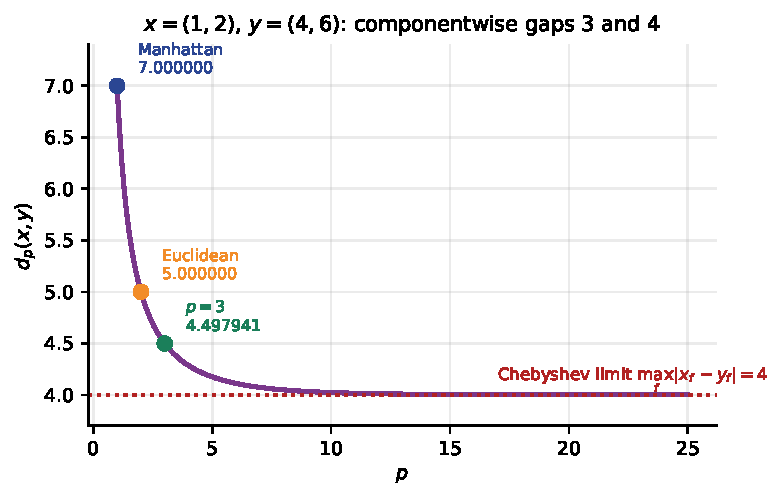
\includegraphics[width=0.55\textwidth]{minkowski_p.pdf}
  \caption{$d_p$ between $(1,2)$ and $(4,6)$ as $p$ varies. Strictly
    decreasing, flattening onto the Chebyshev limit $\max_f|x_f-y_f| = 4$.
    Nothing is special about $p=2$ except habit and differentiability.}
  \label{fig:minkp}
\end{figure}

\begin{figure}[htbp]
  \centering
  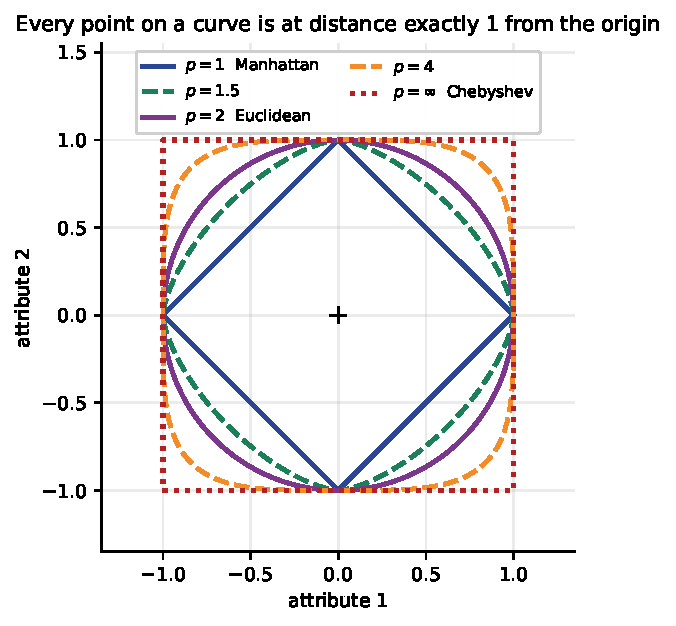
\includegraphics[width=0.42\textwidth]{unit_balls.pdf}
  \caption{The \emph{unit ball} of each metric: the set of points at
    distance exactly $1$ from the centre. $p=1$ is the diamond, $p=2$ the
    circle, $p=\infty$ the square. Along the diagonal --- where the two
    attributes disagree equally --- $p=1$ pulls the boundary in tightest and
    $p=\infty$ pushes it furthest out.}
  \label{fig:balls}
\end{figure}

Figure~\ref{fig:balls} is the picture to remember. Read it like this: every
point on a curve is at distance exactly one from the centre, so a
\emph{fatter} ball means the metric is more \emph{forgiving} of the points
inside it. The four axis-crossings coincide for every $p$ --- a
disagreement of $1$ on a single attribute costs $1$ under every Minkowski
metric. What differs is the diagonal, where the disagreement is spread over
both attributes.

\begin{keyidea}[What $p$ means in one sentence]
$p$ controls how heavily a \emph{single} badly disagreeing attribute is
punished relative to \emph{several} mildly disagreeing ones. Large $p$ says
``one bad attribute makes you far away no matter how well you match on the
rest''; $p=1$ says ``I only care about the total, not how it is
distributed''.
\end{keyidea}

That is not a philosophical point; it changes the answer.

\begin{worked}[$p$ chooses a different neighbour]
Query $q = (0,0)$. Candidate $u = (3,3)$ disagrees a little on both
attributes; candidate $v = (4.5, 0)$ disagrees a lot on one.
\begin{align*}
  d_1(q,u) &= 3+3 = 6.0 & d_1(q,v) &= 4.5 & &\Rightarrow v \text{ is nearer}\\
  d_2(q,u) &= \sqrt{18} = 4.242641 & d_2(q,v) &= 4.5 & &\Rightarrow u
    \text{ is nearer}\\
  d_\infty(q,u) &= 3.0 & d_\infty(q,v) &= 4.5 & &\Rightarrow u \text{ is
    nearer}
\end{align*}
\end{worked}

\begin{codeout}
metric           d(q,u)     d(q,v)   nearest
Manhattan      6.000000   4.500000   v
Euclidean      4.242641   4.500000   u
Minkowski3     3.779763   4.500000   u
Chebyshev      3.000000   4.500000   u
\end{codeout}

Same data, same query, different neighbour. If you are clustering customers
and you want somebody who is slightly unusual on every attribute to count as
more normal than somebody who is wildly unusual on one, you want a large $p$.
If you are clustering sensor readings where the total drift matters and its
distribution does not, you want $p=1$. This is a modelling decision, and it
should be written down.

One further practical point. In very high dimensions Euclidean distances
between random points \emph{concentrate} --- the ratio of the farthest to
the nearest neighbour tends to one --- and $L_1$ degrades more slowly, which
is one reason it is preferred on wide tables. Section~\ref{sec:realdata}
shows Manhattan beating Euclidean on \texttt{wine}.

% =========================================================================
\section{Cosine similarity against Euclidean distance}
\label{sec:cosine}

The one measure in common use that is not in the Minkowski family is
\textbf{cosine similarity}:

\begin{equation}
  \cos(x,y) = \frac{x \cdot y}{\|x\|\,\|y\|}
  = \frac{\sum_f x_f y_f}{\sqrt{\sum_f x_f^2}\,\sqrt{\sum_f y_f^2}}
  \label{eq:cos}
\end{equation}

It is the cosine of the angle between the two vectors, so it ranges over
$[-1,1]$ in general and over $[0,1]$ when the data are non-negative, as
counts and frequencies are. A value of $1$ means the two vectors point in the
same direction; $0$ means they are orthogonal.

\begin{keyidea}[Cosine measures direction and throws away length]
$\cos(x, kx) = 1$ for every $k > 0$. That is the whole character of the
measure. If magnitude carries information, you have just discarded it. If
magnitude is a nuisance --- document length, total spend, image brightness
--- you have just removed it on purpose. There is no third case.
\end{keyidea}

\begin{worked}[The pair on which the two measures disagree]
$A = (1,2)$, \quad $B = (10,20) = 10A$, \quad $C = (2,1)$.
\[
  d(A,B) = \sqrt{(1-10)^2 + (2-20)^2} = \sqrt{81 + 324} = \sqrt{405}
  = 20.124612
\]
\[
  d(A,C) = \sqrt{(1-2)^2 + (2-1)^2} = \sqrt{2} = 1.414214
\]
\[
  \cos(A,B) = \frac{1\cdot10 + 2\cdot20}{\sqrt{1+4}\,\sqrt{100+400}}
  = \frac{50}{\sqrt5 \cdot \sqrt{500}} = \frac{50}{50} = 1.000000
\]
\[
  \cos(A,C) = \frac{1\cdot2 + 2\cdot1}{\sqrt5\,\sqrt5} = \frac{4}{5}
  = 0.800000
\]
\textbf{Euclidean distance says $C$ is $A$'s nearest neighbour, by a factor
of fourteen. Cosine similarity says $B$ \emph{is} $A$.} The angle between
$A$ and $C$ is $\arccos(0.8) = 36.8699^\circ$.
\end{worked}

\begin{codeout}
pair        euclidean   cosine sim
A,B         20.124612     1.000000
A,C          1.414214     0.800000
B,C         20.615528     0.800000
\end{codeout}

\begin{figure}[htbp]
  \centering
  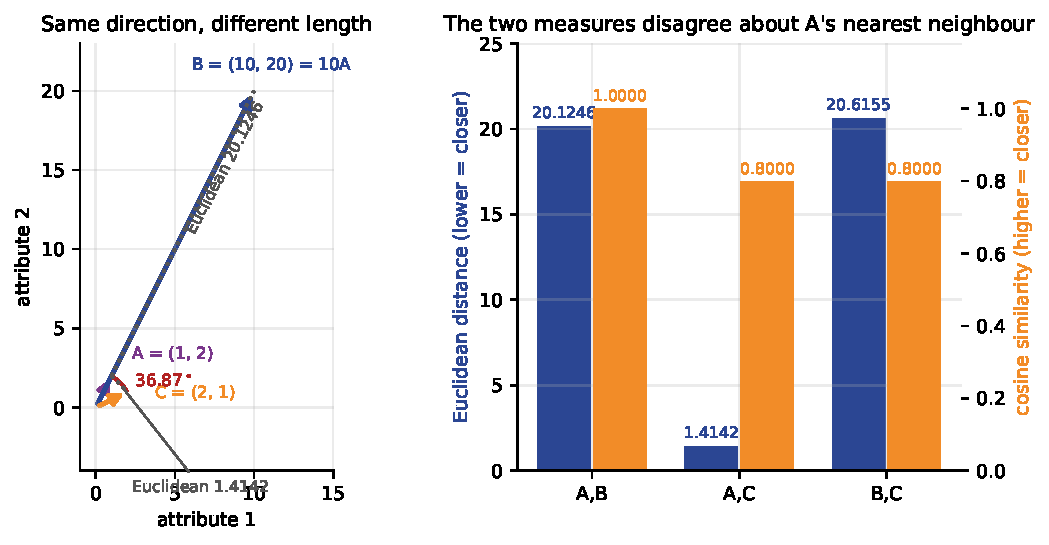
\includegraphics[width=0.76\textwidth]{cosine_vs_euclidean.pdf}
  \caption{The disagreement. Left: $B$ is ten times $A$, so it lies on the
    same ray; $C$ is close to $A$ in the plane but $36.87^\circ$ away in
    angle. Right: the two measures read in opposite directions --- for
    Euclidean, lower is closer; for cosine, higher is closer. The pair
    $A,B$ scores the best possible cosine and nearly the worst Euclidean.}
  \label{fig:cosfig}
\end{figure}

Neither measure is wrong. They answer different questions, and which question
you want is decided by the data, not by the mathematics.

\subsection{The canonical case: text}

\begin{lstlisting}
terms = ["model", "data", "train", "cluster", "the"]
docs = {"d1 short note": [1, 2, 1, 0, 4],
        "d2 long paper": [10, 20, 10, 0, 40],   # exactly 10 x d1
        "d3 short note": [0, 1, 0, 3, 4]}
\end{lstlisting}
\begin{codeout}
doc            doc                euclid     cosine
d1 short note  d2 long paper     42.2137     1.0000
d1 short note  d3 short note      3.4641     0.7526
d2 long paper  d3 short note     43.1972     0.7526
\end{codeout}

\texttt{d2} is \texttt{d1} with every count multiplied by ten --- the same
document, ten times as long. Euclidean distance puts them $42.21$ apart,
\emph{further} than either is from the unrelated \texttt{d3}, and pairs
\texttt{d1} with \texttt{d3} at $3.46$ purely because both are short. Cosine
puts \texttt{d1} and \texttt{d2} at exactly $1.0000$ and gives \texttt{d3}
the same $0.7526$ against both, which is correct: \texttt{d3} is equally
unrelated to a document and to a longer copy of that document.

\begin{caution}[Euclidean distance on raw term counts clusters by length]
This is the single commonest mistake in text clustering. The clusters you get
are ``short documents'', ``medium documents'' and ``long documents'', which
looks like structure and is not. Either use cosine, or normalise the rows,
which the next subsection shows is the same thing.
\end{caution}

\subsection{The bridge: cosine \emph{is} Euclidean on normalised rows}

Write $\hat{a} = a/\|a\|$ for the unit vector in the direction of $a$. Then
$\|\hat a\| = \|\hat b\| = 1$ and

\begin{equation}
  \|\hat a - \hat b\|^2 = \|\hat a\|^2 - 2\,\hat a \cdot \hat b
  + \|\hat b\|^2 = 2 - 2\cos(a,b) = 2\big(1 - \cos(a,b)\big).
  \label{eq:bridge}
\end{equation}

\begin{lstlisting}
uh, vh = u / np.linalg.norm(u), v / np.linalg.norm(v)
print(np.sum((uh - vh)**2), 2 * (1 - cosine_similarity([u], [v])[0, 0]))
\end{lstlisting}
\begin{codeout}
A,B    ||ahat-bhat||^2 = 0.0000000000   2(1-cos) = 0.0000000000   diff 2.22e-16
A,C    ||ahat-bhat||^2 = 0.4000000000   2(1-cos) = 0.4000000000   diff 3.89e-16
B,C    ||ahat-bhat||^2 = 0.4000000000   2(1-cos) = 0.4000000000   diff 1.67e-16
\end{codeout}

Equation~\eqref{eq:bridge} has three consequences worth stating separately.
First, ``use cosine similarity'' and ``$L_2$-normalise every row and then use
Euclidean distance'' are \textbf{the same procedure} --- monotonically
related, so they produce identical rankings and identical clusterings. This
is often the easier one to implement, because every library accepts
Euclidean. Second, $\sqrt{2(1-\cos)}$ is a genuine metric, because it is a
Euclidean distance; this is the repair promised in
Section~\ref{sec:violators}. Third, it explains why $k$-means on
$L_2$-normalised rows is called \emph{spherical} $k$-means and is the
standard way to run $k$-means on text.

\begin{tryit}[Check the bridge on your own numbers]
Take any two vectors, compute $2(1-\cos)$ and the squared Euclidean distance
between their normalised versions, and confirm they agree to machine
precision. Then confirm that $\sqrt{2(1-\cos)}$ satisfies the triangle
inequality on the $A$, $B$, $C$ of Section~\ref{sec:violators}, where
$1-\cos$ did not: you should get
$1.4142 \le 0.7654 + 0.7654 = 1.5307$.
\end{tryit}

% =========================================================================
\section{Binary attributes}
\label{sec:binary}

Now the columns stop being numbers. A \textbf{binary} attribute takes two
values, coded $0$ and $1$. Given two objects $i$ and $j$ described by $p$
binary attributes, everything you can say about their similarity is contained
in four counts.

\begin{center}
\begin{tabular}{llccc}
  \toprule
  & & \multicolumn{2}{c}{object $j$} & \\
  \cmidrule(lr){3-4}
  & & $1$ & $0$ & sum \\
  \midrule
  \multicolumn{1}{l}{object $i$} & $1$ & $q$ & $r$ & $q+r$ \\
                                 & $0$ & $s$ & $t$ & $s+t$ \\
  \midrule
  & sum & $q+s$ & $r+t$ & $p$ \\
  \bottomrule
\end{tabular}
\end{center}

So $q$ counts attributes where both objects are $1$ (a shared
\emph{presence}), $r$ where $i$ has it and $j$ does not, $s$ where $j$ has
it and $i$ does not, and $t$ where both are $0$ (a shared \emph{absence}).
Necessarily $q + r + s + t = p$.

\begin{keyidea}[The one question that decides everything]
\textbf{Is $t$ evidence of similarity?} Two patients who both tested negative
for forty rare diseases --- are they alike? Two shoppers who both failed to
buy any of ten thousand products --- are they alike? Your answer determines
which coefficient you use, and Section~\ref{sec:binflip} shows the two
answers ranking the same pair of pairs in opposite orders.
\end{keyidea}

An attribute is \textbf{symmetric} if its two outcomes are equally
informative and equally frequent in principle: \texttt{gender}, a coin flip,
\texttt{is\_urban}. There is no reason to privilege one code over the other,
and a shared $0$ is exactly as much evidence as a shared $1$. For symmetric
attributes use the \textbf{simple matching coefficient}:

\begin{equation}
  \mathrm{SMC}(i,j) = \frac{q+t}{q+r+s+t},
  \qquad
  d_{\mathrm{SMC}}(i,j) = \frac{r+s}{q+r+s+t}.
  \label{eq:smc}
\end{equation}

An attribute is \textbf{asymmetric} if one outcome is rare and informative
and the other is the default: a positive test result, a purchase, a word
occurring in a document, a gene being expressed. Here a shared $1$ is a
strong signal and a shared $0$ is no signal at all. Use the \textbf{Jaccard
coefficient}:

\begin{equation}
  J(i,j) = \frac{q}{q+r+s},
  \qquad
  d_J(i,j) = \frac{r+s}{q+r+s}.
  \label{eq:jaccard}
\end{equation}

The only difference between \eqref{eq:smc} and \eqref{eq:jaccard} is whether
$t$ appears in the denominator. That single term is the whole examinable
distinction, and it is worth saying out loud: \emph{Jaccard does not merely
down-weight shared absences, it deletes them}.

\subsection{Worked: three patients, six binary tests}

\begin{center}
\begin{tabular}{lcccccc}
  \toprule
  & fever & cough & test1 & test2 & test3 & test4 \\
  \midrule
  Jack & 1 & 0 & 1 & 0 & 0 & 0 \\
  Jim  & 1 & 1 & 0 & 0 & 0 & 0 \\
  Mary & 1 & 0 & 1 & 0 & 1 & 0 \\
  \bottomrule
\end{tabular}
\end{center}

All six attributes are asymmetric: a positive test says something, a negative
one is the default state of a healthy person. We will nevertheless compute
both coefficients, so that the difference is visible.

\begin{worked}[Jack against Mary]
Go attribute by attribute and drop each into one of four buckets.
\begin{itemize}[leftmargin=*,topsep=2pt]
  \item Both $1$: \texttt{fever}, \texttt{test1} $\;\Rightarrow\; q = 2$
  \item Jack $1$, Mary $0$: none $\;\Rightarrow\; r = 0$
  \item Mary $1$, Jack $0$: \texttt{test3} $\;\Rightarrow\; s = 1$
  \item Both $0$: \texttt{cough}, \texttt{test2}, \texttt{test4}
    $\;\Rightarrow\; t = 3$
\end{itemize}
Check: $2 + 0 + 1 + 3 = 6 = p$. \quad Then
\[
  \mathrm{SMC} = \frac{q+t}{p} = \frac{2+3}{6} = \frac{5}{6} = 0.8333,
  \qquad
  J = \frac{q}{q+r+s} = \frac{2}{3} = 0.6667
\]
and the dissimilarities are $1 - 0.8333 = 0.1667$ and
$1 - 0.6667 = 0.3333$.
\end{worked}

\begin{lstlisting}
q = int(np.sum((u == 1) & (v == 1)));  r = int(np.sum((u == 1) & (v == 0)))
s = int(np.sum((u == 0) & (v == 1)));  t = int(np.sum((u == 0) & (v == 0)))
smc = (q + t) / (q + r + s + t);       jac = q / (q + r + s)
\end{lstlisting}
\begin{codeout}
pair           q   r   s   t |   SMC sim   SMC dis |   Jac sim   Jac dis
Jack,Jim       1   1   1   3 |    0.6667    0.3333 |    0.3333    0.6667
Jack,Mary      2   0   1   3 |    0.8333    0.1667 |    0.6667    0.3333
Jim,Mary       1   1   2   2 |    0.5000    0.5000 |    0.2500    0.7500
\end{codeout}

\begin{lstlisting}
from scipy.spatial.distance import hamming, jaccard, pdist, squareform
# scipy dropped the `matching` alias; for 0/1 vectors the simple-matching
# DISSIMILARITY is exactly the Hamming distance.
\end{lstlisting}
\begin{codeout}
Jack,Jim     scipy hamming 0.333333   scipy jaccard 0.666667
Jack,Mary    scipy hamming 0.166667   scipy jaccard 0.333333
Jim,Mary     scipy hamming 0.500000   scipy jaccard 0.750000
For 0/1 vectors scipy's `hamming` -- the proportion of positions
that disagree -- IS the simple-matching dissimilarity (r+s)/p, and
`jaccard` is the Jaccard dissimilarity.  Both are 1 - coefficient.
\end{codeout}

\begin{caution}[\texttt{scipy} has no \texttt{matching} any more, and its
  names mean \emph{distance}]
Older textbooks and older \texttt{scipy} versions offer
\texttt{scipy.spatial.distance.matching}. It was removed. For $0/1$ vectors
\texttt{hamming} is numerically identical to it. Note also that both
\texttt{hamming} and \texttt{jaccard} return \emph{dissimilarities}: if you
want the coefficient, subtract from one. Writing
\texttt{jaccard\_similarity = jaccard(u, v)} is a sign error that will
invert your entire dendrogram.
\end{caution}

Both dissimilarity matrices, side by side:

\begin{codeout}
Jaccard dissimilarity              simple matching dissimilarity
Jack   0.0000  0.6667  0.3333       Jack   0.0000  0.3333  0.1667
Jim    0.6667  0.0000  0.7500       Jim    0.3333  0.0000  0.5000
Mary   0.3333  0.7500  0.0000       Mary   0.1667  0.5000  0.0000
\end{codeout}

On this table the two give the same \emph{ranking} --- Jack and Mary are the
closest pair either way --- but the numbers differ by a factor of two or
more, because simple matching is being paid for four tests that neither
patient had. The next two subsections show the ranking failing too.

\subsection{Shared absences swamp simple matching}
\label{sec:swamp}

Start from two objects that agree on one presence and disagree twice:
$u = 1010$, $v = 1100$, so $q=1$, $r=1$, $s=1$, $t=1$. Now append $k$
attributes on which both objects are $0$.

\begin{codeout}
       k    SMC sim Jaccard sim
       0     0.5000     0.3333
       4     0.7500     0.3333
      16     0.9000     0.3333
      96     0.9800     0.3333
     996     0.9980     0.3333
\end{codeout}

Jaccard never moves. Simple matching walks steadily to $1$.

\begin{keyidea}[The market-basket argument]
Adding a thousand products that \textbf{nobody bought} to your catalogue
cannot make two shoppers more alike. But simple matching says it does: two
shoppers who bought entirely different things become $99.8\%$ similar. On
sparse, asymmetric data --- baskets, documents, symptom checklists,
click logs --- simple matching is not a conservative default, it is simply
the wrong measure.
\end{keyidea}

\subsection{The two coefficients can rank two pairs in opposite orders}
\label{sec:binflip}

\begin{worked}[A genuine reversal]
Ten binary attributes, two pairs of patients.
\begin{center}
\begin{tabular}{lllcccc}
  \toprule
  & & & $q$ & $r$ & $s$ & $t$ \\
  \midrule
  pair 1 & $u = 1100000000$ & $v = 1010000000$ & 1 & 1 & 1 & 7 \\
  pair 2 & $u = 1111111100$ & $v = 1111110011$ & 6 & 2 & 2 & 0 \\
  \bottomrule
\end{tabular}
\end{center}
\[
  \mathrm{SMC}_1 = \frac{1+7}{10} = 0.8000, \qquad
  \mathrm{SMC}_2 = \frac{6+0}{10} = 0.6000
  \qquad \Rightarrow \text{pair 1 is more similar}
\]
\[
  J_1 = \frac{1}{1+1+1} = 0.3333, \qquad
  J_2 = \frac{6}{6+2+2} = 0.6000
  \qquad \Rightarrow \text{pair 2 is more similar}
\]
\end{worked}

\begin{codeout}
simple matching: pair 1 (0.8000) is more similar than pair 2 (0.6000)
Jaccard:         pair 2 (0.6000) is more similar than pair 1 (0.3333)
They disagree about which pair of patients is more alike.  Neither
is wrong; they answer different questions.
\end{codeout}

\begin{figure}[htbp]
  \centering
  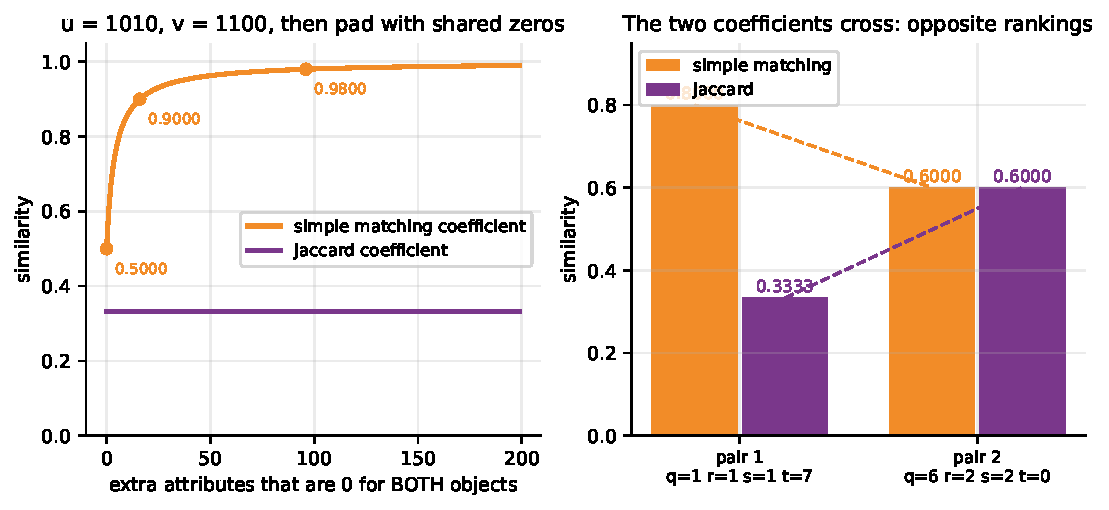
\includegraphics[width=0.84\textwidth]{binary_smc_jaccard.pdf}
  \caption{Left: padding with shared zeros drives the simple matching
    coefficient to $1$ while Jaccard stays flat at $0.333333$. Right: the
    two coefficients cross --- simple matching ranks pair 1 above pair 2,
    Jaccard ranks pair 2 above pair 1.}
  \label{fig:binfig}
\end{figure}

This is not a rounding difference; it is a reversal. Any clustering built on
these two coefficients will put different patients in the same group. The
decision ``is a shared absence evidence?'' is made once, before any algorithm
runs, and it decides the answer.

\subsection{The $0/1$ coding is not a free choice}

\begin{codeout}
u = [1 1 1 0 0]   v = [1 0 0 0 0]
   q=1 r=2 s=0 t=2 ->  Jaccard sim 0.3333    SMC sim 0.6000
now swap the meaning of 0 and 1 on every attribute:
u = [0 0 0 1 1]   v = [0 1 1 1 1]
   q=2 r=0 s=2 t=1 ->  Jaccard sim 0.5000    SMC sim 0.6000
\end{codeout}

Simple matching is unchanged at $0.6000$: it is symmetric in the two codes,
which is precisely what ``symmetric attribute'' means. Jaccard moves from
$0.3333$ to $0.5000$, because it counts only whichever value you happened to
call $1$.

\begin{caution}[Decide which outcome is ``present'' before you compute]
For an asymmetric attribute the $1$ must be the rare, informative outcome. If
your data file codes ``no complication'' as $1$ and ``complication'' as $0$,
you must flip it before computing Jaccard, or you will be measuring how
similarly healthy your patients are.
\end{caution}

Two relatives worth naming. The \textbf{Dice} coefficient
$2q/(2q+r+s)$ is Jaccard with shared presences double-weighted, and is
monotonically related to it, so it gives the same ranking. The \textbf{Rand
index} is the simple matching coefficient applied to \emph{pairs of objects}
rather than attributes, and is the basis of the adjusted Rand index used in
Section~\ref{sec:realdata}.

% =========================================================================
\section{Nominal attributes}
\label{sec:nominal}

A \textbf{nominal} attribute takes one of $M > 2$ unordered values:
\texttt{colour} $\in$ \{red, blue, green\}, \texttt{city},
\texttt{department}. There is no order and no arithmetic. The standard
dissimilarity is the \textbf{mismatch ratio}:

\begin{equation}
  d(i,j) = \frac{p - m}{p}
  \label{eq:nominal}
\end{equation}

where $p$ is the number of nominal attributes and $m$ is the number on which
$i$ and $j$ take the same value. It ranges over $[0,1]$, and it is a metric
(it is a scaled Hamming distance).

\begin{worked}[Three objects, three nominal attributes]
\begin{center}
\begin{tabular}{lccc}
  \toprule
  & colour & shape & material \\ \midrule
  A & red & round & wood \\
  B & red & square & wood \\
  C & blue & square & metal \\ \bottomrule
\end{tabular}
\qquad
\begin{tabular}{lccc}
  \toprule
  pair & $p$ & $m$ & $(p-m)/p$ \\ \midrule
  A,B & 3 & 2 & $1/3 = 0.333333$ \\
  A,C & 3 & 0 & $3/3 = 1.000000$ \\
  B,C & 3 & 1 & $2/3 = 0.666667$ \\ \bottomrule
\end{tabular}
\end{center}
$A$ and $B$ agree on colour and material and differ on shape, so $m = 2$.
$A$ and $C$ agree on nothing, so $m = 0$ and the dissimilarity is at its
maximum.
\end{worked}

\subsection{The one-hot alternative, and when it agrees}

The other standard approach is to replace each nominal attribute by one
binary dummy column per level --- \textbf{one-hot encoding} --- and then use
an ordinary numeric distance. Does that give the same answer?

\begin{codeout}
columns: colour=blue, colour=red, shape=round, shape=square,
         material=metal, material=wood
  A        0  1  1  0  0  1
  B        0  1  0  1  0  1
  C        1  0  0  1  1  0

pair        (p-m)/p      L1/(2p)   L1 one-hot   L2 one-hot
A,B        0.333333     0.333333     2.000000     1.414214
A,C        1.000000     1.000000     6.000000     2.449490
B,C        0.666667     0.666667     4.000000     2.000000
\end{codeout}

Each mismatched attribute flips exactly \emph{two} dummy columns: the level
$i$ has goes from $1$ to $0$ and the level $j$ has goes from $0$ to $1$. So
$L_1$ on the dummies is exactly $2(p-m)$, and

\begin{equation}
  \frac{L_1(\text{one-hot})}{2p} = \frac{2(p-m)}{2p} = \frac{p-m}{p}.
  \label{eq:onehotl1}
\end{equation}

\textbf{With $L_1$, one-hot encoding reproduces the mismatch ratio exactly},
to the last digit, as the table shows.

With $L_2$ it does not. Squared Euclidean on the dummies is also $2(p-m)$, so
$L_2 = \sqrt{2(p-m)}$: monotone in the same quantity, therefore
\emph{rank-equivalent}, but not proportional. The ratio between the largest
and smallest non-zero mismatch scores is $1.000000/0.333333 = 3.0000$ under
\eqref{eq:nominal} but only $2.449490/1.414214 = 1.7321$ under $L_2$.
Euclidean on dummies compresses the gaps by a square root.

\begin{caution}[Rank-equivalent is not the same as equal]
For a single clustering run on nominal data alone, a monotone
re-parameterisation is harmless: single and complete linkage depend only on
the order of the distances. But the moment you \emph{combine} the nominal
part with a numeric part --- as Gower does in Section~\ref{sec:mixed} --- the
compression matters, because the two parts are being added together and the
square root has changed their relative weight.
\end{caution}

\subsection{Where one-hot stops agreeing entirely}

The equivalence above assumed the dummy columns are used raw. If you
standardise them --- and many pipelines standardise every column by reflex
--- the agreement collapses, because a dummy column with proportion $\pi$ has
standard deviation $\sqrt{\pi(1-\pi)}$, so a \emph{rare} level gets a large
weight.

\begin{codeout}
20 rows, three nominal attributes.  Level frequencies:
  f1: {'a': 10, 'b': 10}
  f2: {'P': 10, 'Q': 10}
  f3: {'u': 19, 'w': 1}
column standard deviations (sqrt(pi(1-pi)) for a dummy):
  0.5000  0.5000  0.5000  0.5000  0.2179  0.2179

obj  f1   f2   f3   | mismatches |      (p-m)/p |     z-dummy L2
x0   a    P    u    |          0 |     0.000000 |       0.000000
xA   a    P    w    |          1 |     0.333333 |       6.488857
xB   b    Q    u    |          2 |     0.666667 |       4.000000
\end{codeout}

The mismatch ratio says \texttt{xA}, which differs from the query on one
attribute out of three, is nearer than \texttt{xB}, which differs on two.
Standardised dummies say the opposite. The arithmetic is easy to check by
hand: a mismatch on a balanced two-level attribute contributes
$2/0.5^2 = 8$ to the squared distance, so \texttt{xB} scores
$\sqrt{8+8} = 4.0000$; a mismatch on the level occurring once in twenty
contributes $2/0.2179^2 = 42.105$, so \texttt{xA} scores $6.488857$.

\begin{keyidea}[A rare category buys influence nobody granted it]
Standardising one-hot columns makes the distance depend on how \emph{common}
each category is, not only on whether the objects agree. Sometimes that is
what you want --- agreeing on a rare category really is more informative than
agreeing on a common one, and that is the intuition behind inverse-document
frequency. But it is a modelling decision, and if you did it by putting
\texttt{StandardScaler} in front of everything, you did not make it, your
pipeline did.
\end{keyidea}

% =========================================================================
\section{Ordinal attributes}
\label{sec:ordinal}

An \textbf{ordinal} attribute has $M$ values with a meaningful order but no
meaningful spacing: \{poor, fair, good, very good, excellent\},
\{junior, mid, senior\}, a five-star rating, a pain scale. Treating it as
nominal throws away the order; treating the raw codes $1,\dots,M$ as numbers
makes the answer depend on how many levels the scale happens to have.

The standard fix is to replace the rank $r_{if} \in \{1,\dots,M_f\}$ by

\begin{equation}
  z_{if} = \frac{r_{if} - 1}{M_f - 1} \in [0,1]
  \label{eq:ordinal}
\end{equation}

and then treat $z$ as a numeric attribute. Dividing by $M_f - 1$ is what
makes scales of different length commensurable: a three-level attribute and a
seven-level attribute both span exactly $[0,1]$, so neither dominates a sum
simply by having more categories.

\begin{codeout}
M = 5
  r=1  poor       -> (1-1)/(5-1) = 0.0000
  r=2  fair       -> (2-1)/(5-1) = 0.2500
  r=3  good       -> (3-1)/(5-1) = 0.5000
  r=4  very good  -> (4-1)/(5-1) = 0.7500
  r=5  excellent  -> (5-1)/(5-1) = 1.0000
M = 3
  r=1  junior     -> (1-1)/(3-1) = 0.0000
  r=2  mid        -> (2-1)/(3-1) = 0.5000
  r=3  senior     -> (3-1)/(3-1) = 1.0000
\end{codeout}

\begin{worked}[Two ordinal attributes]
Three staff, rated on satisfaction ($M=5$) and grade ($M=3$).
\begin{center}
\begin{tabular}{lllcc}
  \toprule
  & rating & grade & $z_1$ & $z_2$ \\ \midrule
  $P$ & excellent & senior & 1.0000 & 1.0000 \\
  $Q$ & good      & junior & 0.5000 & 0.0000 \\
  $R$ & fair      & mid    & 0.2500 & 0.5000 \\ \bottomrule
\end{tabular}
\end{center}
For $P$ and $Q$: $|1.00 - 0.50| = 0.50$ and $|1.00 - 0.00| = 1.00$, so the
Euclidean distance is $\sqrt{0.25 + 1.00} = \sqrt{1.25} = 1.118034$ and the
mean absolute gap --- the form Gower uses --- is
$(0.50 + 1.00)/2 = 0.750000$.
\end{worked}

\begin{codeout}
pair        |dz1|      |dz2|       euclid    mean |dz|
P,Q        0.5000     1.0000     1.118034     0.750000
P,R        0.7500     0.5000     0.901388     0.625000
Q,R        0.2500     0.5000     0.559017     0.375000
the last column is the form Gower uses; the ranking is the same
\end{codeout}

\begin{figure}[htbp]
  \centering
  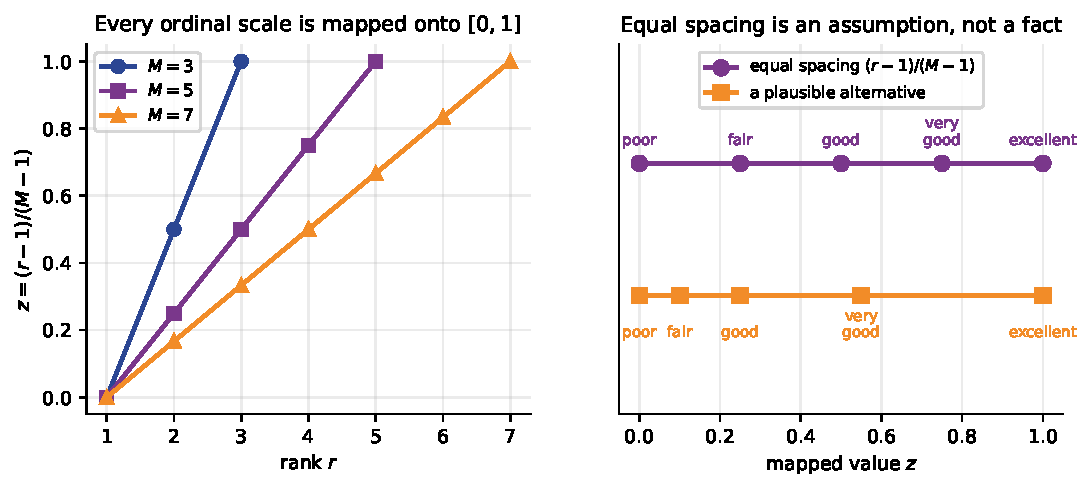
\includegraphics[width=0.80\textwidth]{ordinal_map.pdf}
  \caption{Left: $(r-1)/(M-1)$ places any ordinal scale on $[0,1]$
    regardless of its length. Right: the equal-spacing assumption, against
    one plausible alternative for the same five labels.}
  \label{fig:ordfig}
\end{figure}

\begin{caution}[Equal spacing is an assumption, not a fact]
Equation~\eqref{eq:ordinal} asserts that the step from \emph{poor} to
\emph{fair} is exactly as large as the step from \emph{very good} to
\emph{excellent}: both are $0.2500$. Few real rating scales behave that way.
Customers who write ``excellent'' are often a very different population from
those who write ``very good'', while ``poor'' and ``fair'' are nearly
interchangeable. If you have domain knowledge about the spacing, encode it;
if you do not, use \eqref{eq:ordinal} and \emph{say in your report that you
assumed equal spacing}. It is a defensible default and an indefensible
silence.
\end{caution}

% =========================================================================
\section{Mixed attribute types: the Gower dissimilarity}
\label{sec:mixed}

Real tables are not all one type. A recruitment table has age (numeric),
degree (ordinal), city (nominal) and a set of yes/no flags (binary, some
symmetric and some not). The standard answer is due to Gower: compute a
per-attribute dissimilarity in $[0,1]$ for each column, then take a weighted
average.

\begin{equation}
  d(i,j) = \frac{\displaystyle\sum_{f=1}^{p} \delta_f^{(ij)}\, d_f^{(ij)}}
                {\displaystyle\sum_{f=1}^{p} \delta_f^{(ij)}}
  \label{eq:gower}
\end{equation}

The per-attribute term $d_f^{(ij)}$ depends on the attribute's type:

\begin{itemize}[leftmargin=*]
  \item \textbf{numeric}: $d_f = |x_{if} - x_{jf}| \,/\, R_f$, where
    $R_f = \max_f - \min_f$ is the range over all objects. Dividing by the
    range is what puts it in $[0,1]$.
  \item \textbf{nominal} or \textbf{symmetric binary}: $d_f = 0$ if the two
    objects agree, $1$ otherwise.
  \item \textbf{asymmetric binary}: $d_f = 0$ if they agree, $1$ otherwise
    --- same rule, but see the indicator below.
  \item \textbf{ordinal}: map to $z$ by \eqref{eq:ordinal}, then
    $d_f = |z_{if} - z_{jf}|$.
\end{itemize}

The indicator $\delta_f^{(ij)}$ is where the type information really lives.
It is $0$ --- meaning ``skip this attribute for this pair'' --- in exactly
two situations: when $x_{if}$ or $x_{jf}$ is \textbf{missing}, and when the
attribute is \textbf{asymmetric binary and both objects are $0$}. Otherwise
it is $1$.

\begin{keyidea}[A skipped attribute leaves both sums]
Setting $\delta_f = 0$ removes the attribute from the numerator
\emph{and} from the denominator. It is not the same as scoring $d_f = 0$,
which would count the attribute as evidence of similarity. This is the
Jaccard idea from Section~\ref{sec:binary} embedded inside a general
formula: a shared absence on an asymmetric attribute is not evidence, so it
does not get a vote.
\end{keyidea}

\subsection{Worked: four applicants, four attribute types}

\begin{center}
\begin{tabular}{lrrllccc}
  \toprule
  id & age & exp & degree & city & car & python & patent \\
  \midrule
  A & 24 & 2 & BTech & Dehradun & 1 & 1 & 0 \\
  B & 29 & 6 & MTech & Dehradun & 0 & 1 & 0 \\
  C & 41 & 18 & PhD & Mumbai & 1 & 0 & 1 \\
  D & 26 & 3 & BTech & Delhi & 0 & 1 & 0 \\
  \bottomrule
\end{tabular}
\end{center}

Age and experience in years are numeric; degree is ordinal with
BTech $<$ MTech $<$ PhD; city is nominal; \texttt{car}, \texttt{python} and
\texttt{patent} are asymmetric binary --- owning a car, knowing Python and
holding a patent are all informative facts, whereas not doing so is the
default.

\begin{codeout}
ranges used to normalise the numeric attributes:
  age        max 41 - min 24 = 17
  experience max 18 - min 2 = 16
ordinal map: BTech 0.0, MTech 0.5, PhD 1.0
\end{codeout}

\begin{worked}[$d(A,B)$, attribute by attribute]
\begin{center}
\begin{tabular}{lrrr}
  \toprule
  attribute $f$ & $\delta_f$ & $d_f$ & $\delta_f d_f$ \\
  \midrule
  age (numeric) & 1 & $5/17 = 0.294118$ & 0.294118 \\
  experience (numeric) & 1 & $4/16 = 0.250000$ & 0.250000 \\
  degree (ordinal) & 1 & $|0 - 0.5| = 0.500000$ & 0.500000 \\
  city (nominal) & 1 & both Dehradun, $0.000000$ & 0.000000 \\
  car (asym binary) & 1 & $1$ vs $0$, $1.000000$ & 1.000000 \\
  python (asym binary) & 1 & both $1$, $0.000000$ & 0.000000 \\
  patent (asym binary) & \textbf{0} & both $0$: skipped & 0.000000 \\
  \midrule
  SUM & \textbf{6} & & \textbf{2.044118} \\
  \bottomrule
\end{tabular}
\end{center}
\[
  d(A,B) = \frac{2.044118}{6} = \mathbf{0.340686}
\]
\end{worked}

\begin{codeout}
attribute f            delta_f        d_f      delta*d
age (numeric)                1   0.294118     0.294118
experience (numeric)         1   0.250000     0.250000
degree (ordinal)             1   0.500000     0.500000
city (nominal)               1   0.000000     0.000000
car (asym binary)            1   1.000000     1.000000
python (asym binary)         1   0.000000     0.000000
patent (asym binary)         0   0.000000     0.000000
SUM                          6                2.044118
d = 2.044118 / 6 = 0.340686
\end{codeout}

The pair $B,D$ is the one that shows the indicator doing real work: neither
owns a car and neither holds a patent, so \emph{two} attributes are skipped
and the denominator is $5$, not $7$.

\begin{codeout}
attribute f            delta_f        d_f      delta*d
age (numeric)                1   0.176471     0.176471
experience (numeric)         1   0.187500     0.187500
degree (ordinal)             1   0.500000     0.500000
city (nominal)               1   1.000000     1.000000
car (asym binary)            0   0.000000     0.000000
python (asym binary)         1   0.000000     0.000000
patent (asym binary)         0   0.000000     0.000000
SUM                          5                1.863971
d = 1.863971 / 5 = 0.372794
\end{codeout}

Divide by $7$ instead and you get $0.266282$: a different answer, and a wrong
one. It would say that $B$ and $D$ are the closest pair in the whole table
purely because they both fail to own things.

\begin{codeout}
             A         B         C         D
A     0.000000  0.340686  0.857143  0.363358
B     0.340686  0.000000  0.850840  0.372794
C     0.857143  0.850840  0.000000  0.974265
D     0.363358  0.372794  0.974265  0.000000

nearest to A: B (0.340686)  <  D (0.363358)  <  C (0.857143)
\end{codeout}

\begin{figure}[htbp]
  \centering
  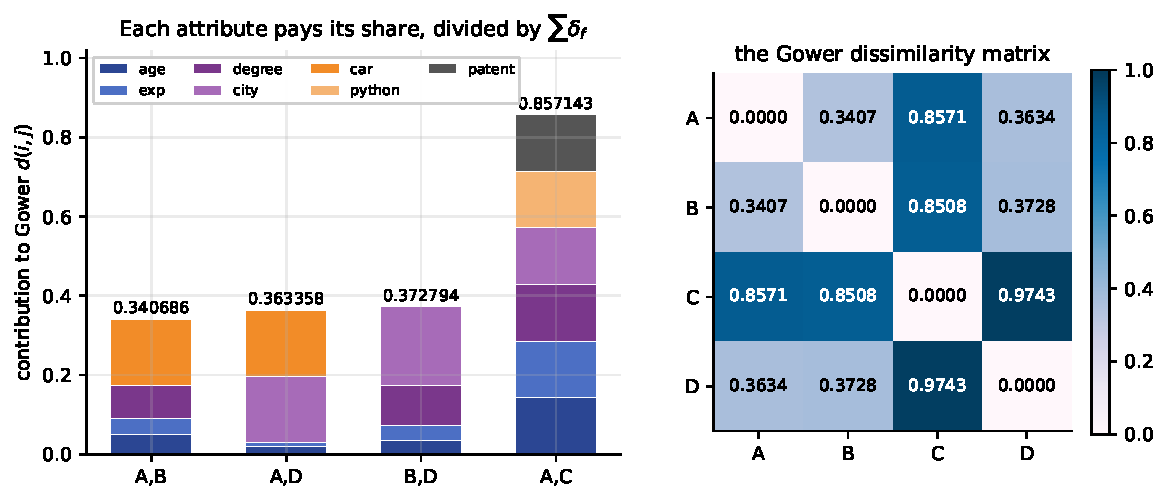
\includegraphics[width=0.84\textwidth]{mixed_gower.pdf}
  \caption{Left: each attribute's contribution $\delta_f d_f / \sum\delta_f$
    to four of the pairwise Gower dissimilarities. Right: the full $4\times4$
    matrix. $B$ and $D$ are separated by only $0.022672$ in their distance
    to $A$.}
  \label{fig:gowerfig}
\end{figure}

\subsection{What happens if you skip the type handling}

The tempting shortcut is to label-encode the nominal column, treat everything
as numeric, and run Euclidean distance.

\begin{lstlisting}
E = np.array([[r[1], r[2], DEGREE.index(r[3]), cities.index(r[4]),
               r[5], r[6], r[7]] for r in APPL], float)
Draw = squareform(pdist(E, "euclidean"))
Dz   = squareform(pdist(StandardScaler().fit_transform(E), "euclidean"))
\end{lstlisting}
\begin{codeout}
             A         B         C         D
A       0.0000    6.5574   23.5584    2.6458
B       6.5574    0.0000   17.2047    4.4721
C      23.5584   17.2047    0.0000   21.4009
D       2.6458    4.4721   21.4009    0.0000
nearest to A, raw Euclidean : D
nearest to A, z-scored      : D
nearest to A, Gower         : B
\end{codeout}

Two things went wrong and both are invisible in the output. First, the raw
distance is dominated by \texttt{experience}, whose range is sixteen years,
while every binary flag can contribute at most one. Second --- and this is
the one that will cost you marks --- \texttt{LabelEncoder} turned
\texttt{city} into a number on which Delhi $(0) <$ Dehradun $(1) <$ Mumbai
$(2)$, so the encoding asserts that Delhi is exactly as far from Dehradun as
Dehradun is from Mumbai, and half as far from Dehradun as from Mumbai. Nobody
chose that ordering. It came from alphabetical sorting.

\begin{caution}[\texttt{LabelEncoder} on a nominal column]
This is the commonest silent bug in student clustering code. If a column has
no order, it must be one-hot encoded, handled by a Gower-style rule, or
dropped. Label-encoding invents an order and a spacing, and the clustering
will faithfully reflect the invention.
\end{caution}

\begin{tryit}[Finish the matrix by hand]
Compute $d(A,C)$ and $d(C,D)$ for the applicant table, showing every
$\delta_f$. You should get $0.857143$ and $0.974265$. Note that $d(A,C)$
has denominator $7$ --- no attribute is skipped, because \texttt{patent}
is $0$ for $A$ and $1$ for $C$.
\end{tryit}

% =========================================================================
\section{Standardisation changes the answer}
\label{sec:standard}

Everything above assumed the numeric columns were commensurable. They almost
never are. A table with an annual fee in rupees and a usage ratio in $[0,1]$
has one column whose values are around $50\,000$ and one whose values are
around $0.5$; squared differences in the first are a hundred million times
larger than squared differences in the second, so the second column simply
does not participate in the distance.

\begin{worked}[Ten customers, two columns]
\begin{center}
\begin{tabular}{rrr}
  \toprule
  row & fee (rupees) & usage \\ \midrule
  0 & 48000 & 0.30 \\
  1 & 50000 & 0.50 \\
  2 & 50300 & 0.90 \\
  3 & 52000 & 0.51 \\
  4 & 49500 & 0.42 \\
  \bottomrule
\end{tabular}
\qquad
\begin{tabular}{rrr}
  \toprule
  row & fee (rupees) & usage \\ \midrule
  5 & 51000 & 0.66 \\
  6 & 47000 & 0.25 \\
  7 & 53000 & 0.72 \\
  8 & 50800 & 0.88 \\
  9 & 49000 & 0.35 \\
  \bottomrule
\end{tabular}
\end{center}
Query is row 1. Row 2 differs by $300$ rupees and $0.40$ of usage;
row 4 differs by $500$ rupees and $0.08$ of usage.
\[
  d_{\text{raw}}(1,2) = \sqrt{300^2 + 0.40^2} = 300.000267, \qquad
  d_{\text{raw}}(1,4) = \sqrt{500^2 + 0.08^2} = 500.000006
\]
Row 2 wins. The usage gap of $0.40$ changed the answer by $0.000267$.
\end{worked}

\begin{codeout}
fee    mean   50060.00  sd  1701.2936  range       6000
usage  mean     0.5490  sd     0.2204  range       0.65

 row          fee    usage |        d raw   d z-scored
   0        48000     0.30 |  2000.000010     1.484995
   1        50000     0.50 |     0.000000     0.000000   <- query
   2        50300     0.90 |   300.000267     1.823190
   3        52000     0.51 |  2000.000000     1.176451
   4        49500     0.42 |   500.000006     0.467002
   5        51000     0.66 |  1000.000013     0.934004
   6        47000     0.25 |  3000.000010     2.096605
   7        53000     0.72 |  3000.000008     2.026219
   8        50800     0.88 |   800.000090     1.786892
   9        49000     0.35 |  1000.000011     0.899201

nearest neighbour, raw      : row 2  (d = 300.000267)
nearest neighbour, z-scored : row 4  (d = 0.467002)
share of raw squared distance carried by fee, over the 9 others:
  min 0.999998   max 1.000000   mean 1.000000
\end{codeout}

\begin{figure}[htbp]
  \centering
  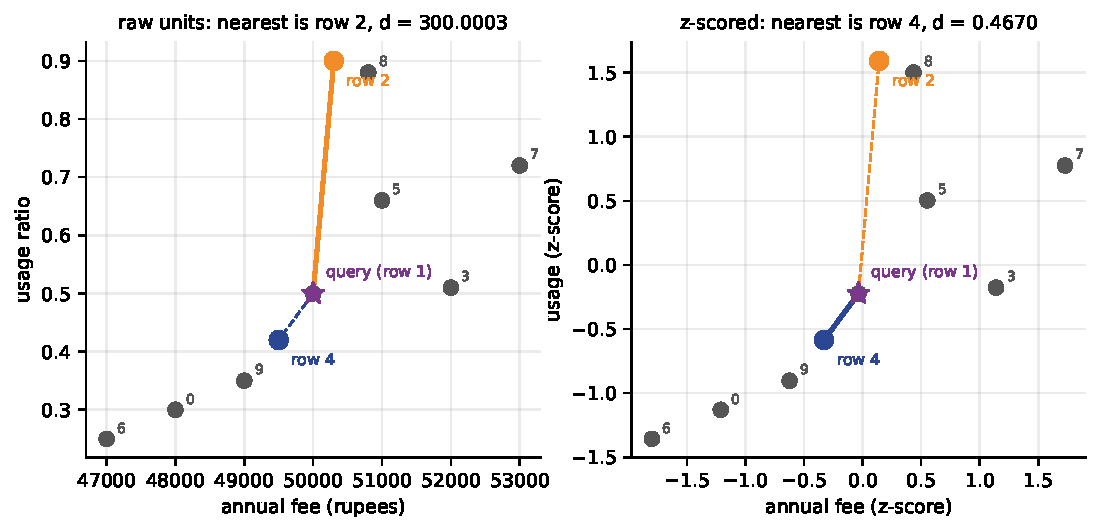
\includegraphics[width=0.84\textwidth]{standardisation_flip.pdf}
  \caption{The same ten customers, the same query, the same metric. Only the
    units changed, and the nearest neighbour changed identity from row 2 to
    row 4.}
  \label{fig:stdflip}
\end{figure}

\begin{keyidea}[An unscaled distance is a distance in the biggest column]
The share of raw squared distance carried by the fee column, averaged over
all nine other rows, is $1.000000$ to six decimal places. The usage column
was not consulted. Whenever your columns have different units, ``Euclidean
distance'' means ``difference in whichever column happens to have the largest
numbers'' --- an answer that changes if somebody records the fee in thousands
of rupees instead.
\end{keyidea}

This is not a property of contrived tables.

\begin{lstlisting}
X = load_wine().data;  Xz = StandardScaler().fit_transform(X)
# for each row: is the argmin over raw distances the same row as over z?
\end{lstlisting}
\begin{codeout}
wine: 178 rows, 13 features
rows whose nearest neighbour CHANGES IDENTITY under z-scoring:
  168 / 178  (94.4%)
row 0 nearest, raw      : row  54  d =    10.3928  class 0
row 0 nearest, z-scored : row  20  d =     1.2879  class 0
one column, proline (variance 98609.6), carries 0.997738 of the total
raw squared distance.
\end{codeout}

On \texttt{wine}, $94.4\%$ of rows get a different nearest neighbour when you
standardise. This is the $k$-NN lecture's scaling lesson arriving from the
other direction: there it changed a classifier's accuracy, here it changes
which object is nearest, and those are the same fact.

\subsection{z-score against mean absolute deviation}

The default standardisation is the \textbf{z-score}, subtract the mean and
divide by the standard deviation:
$z_{if} = (x_{if} - \mu_f)/\sigma_f$. The textbook alternative is to divide
instead by the \textbf{mean absolute deviation}

\begin{equation}
  s_f = \frac{1}{n}\sum_{i=1}^{n} \big| x_{if} - \mu_f \big|,
  \qquad
  z_{if} = \frac{x_{if} - \mu_f}{s_f}.
  \label{eq:mad}
\end{equation}

The point is robustness. $\sigma_f$ is built from \emph{squared} deviations,
so a single extreme value inflates it out of proportion; $s_f$ uses absolute
deviations, so it is inflated only linearly.

\begin{worked}[$x = 1, 2, 3, 4, 100$]
Mean $\mu = 110/5 = 22$. Deviations: $-21, -20, -19, -18, +78$.
\[
  \sigma = \sqrt{\frac{21^2 + 20^2 + 19^2 + 18^2 + 78^2}{5}}
  = \sqrt{\frac{441+400+361+324+6084}{5}} = \sqrt{\frac{7610}{5}}
  = \sqrt{1522} = 39.012818
\]
\[
  s = \frac{21+20+19+18+78}{5} = \frac{156}{5} = 31.200000
\]
The gap between $x=1$ and $x=2$ after scaling is $1/\sigma = 0.025633$ under
the z-score and $1/s = 0.032051$ under \eqref{eq:mad}: the four ordinary
points keep $25.0\%$ more separation from each other.
\end{worked}

\begin{codeout}
mean 22.0000    sd 39.012818    mean absolute deviation 31.200000
         x    (x-mean)/sd   (x-mean)/mad
       1.0      -0.538285      -0.673077
       2.0      -0.512652      -0.641026
       3.0      -0.487019      -0.608974
       4.0      -0.461387      -0.576923
     100.0       1.999343       2.500000

gap between x=1 and x=2 after scaling:
  by sd  0.025633       by mad  0.032051       ratio 1.2504
the outlier's own score:  sd 1.9993   mad 2.5000
\end{codeout}

\begin{figure}[htbp]
  \centering
  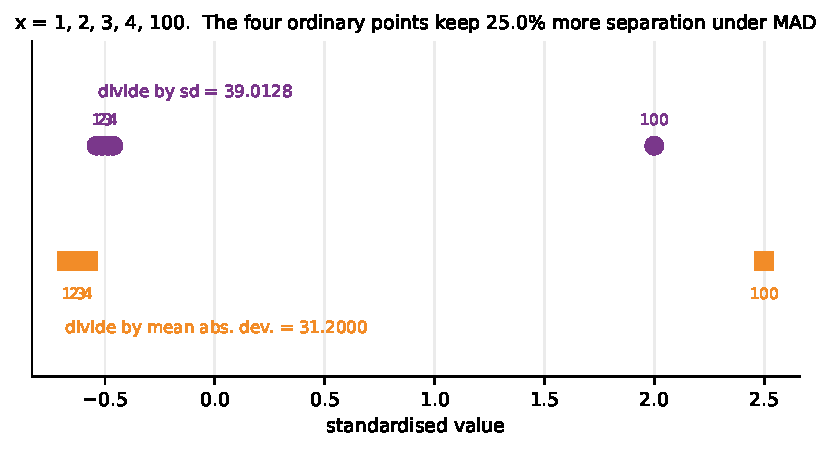
\includegraphics[width=0.70\textwidth]{zscore_vs_mad.pdf}
  \caption{The same five values under both standardisations. Dividing by
    $\sigma$, which the outlier inflated quadratically, crushes the four
    ordinary points together; dividing by the mean absolute deviation leaves
    them further apart and pushes the outlier further out.}
  \label{fig:zmad}
\end{figure}

Notice both halves of the effect. The ordinary points spread out
\emph{and} the outlier's own score grows, from $1.9993$ to $2.5000$. Under
the z-score the outlier is barely two standard deviations out, which is
almost unremarkable; under \eqref{eq:mad} it is where it belongs.

For a Gaussian column the two agree up to a constant:
$\sigma/s \to \sqrt{\pi/2} = 1.2533$. So the \emph{ratio} $\sigma/s$ is a
tail-weight diagnostic, and it is worth computing before you decide.

\begin{codeout}
dataset        column                             sd        mad   sd/mad
breast_cancer  area error                    45.4510    27.1965   1.6712
breast_cancer  concavity error                0.0302     0.0186   1.6208
breast_cancer  fractal dimension error        0.0026     0.0017   1.5886
breast_cancer  perimeter error                2.0201     1.3325   1.5160
breast_cancer  radius error                   0.2771     0.1893   1.4638
...
wine           od280/od315_of_diluted_wines     0.7080     0.6117   1.1573
iris           petal width (cm)               0.7597     0.6581   1.1543
iris           petal length (cm)              1.7594     1.5627   1.1258
\end{codeout}

\begin{caution}[Reported honestly: on \texttt{wine} and \texttt{iris} it
  barely matters]
Every \texttt{wine} and \texttt{iris} column sits within a few per cent of
$1.2533$, so on those two datasets the choice between $\sigma$ and $s$
changes almost nothing. The gap opens on the \texttt{breast\_cancer} ``error''
columns, where $\sigma$ is up to $1.67$ times $s$ because a handful of
extreme patients dominate the squared deviations. \textbf{MAD scaling earns
its keep when the tail is real, not on every dataset.} Do not write in a
report that it improved your clustering unless you measured that it did.
\end{caution}

A third option worth knowing is \texttt{RobustScaler}, which centres on the
median and divides by the interquartile range: more robust than either of the
above, and the right default when you expect contamination rather than merely
a heavy tail.

% =========================================================================
\section{Cluster centroid, medoid, and the distance between two clusters}
\label{sec:centroid}

Once objects are grouped, two further quantities are needed: a summary of
where a cluster \emph{is}, and a distance between two clusters. Both feed
directly into the next two lectures.

\subsection{Three ways to name the middle}

The \textbf{centroid} is the componentwise mean
$\bar{c} = \frac1n \sum_i x_i$. It minimises $\sum_i \|x_i - c\|^2$, it
requires numeric attributes, and it is usually \emph{not} one of the data
points.

The \textbf{medoid} is the object in the cluster with the smallest total
distance to the others. It \emph{is} a data point, and it needs nothing but
the dissimilarity matrix --- so it works with Gower distances, string edit
distances, anything.

The \textbf{mode} is the most frequent value per attribute, used for purely
nominal data where a mean is meaningless. (There is no ``average colour''.)

\begin{keyidea}[This distinction is $k$-means against $k$-medoids]
$k$-means represents a cluster by its centroid, so it needs numeric data and
squared Euclidean distance. $k$-medoids represents a cluster by an actual
object, so it works with any dissimilarity matrix and is resistant to
outliers, at the cost of being much slower. That is the whole difference, and
it is why $k$-medoids can cluster the mixed-type applicant table of
Section~\ref{sec:mixed} and $k$-means cannot.
\end{keyidea}

\begin{worked}[Centroid and medoid of a three-point cluster]
$A = \{(1,1),\,(2,1),\,(1,2)\}$.
\[
  \bar{c} = \left(\frac{1+2+1}{3}, \frac{1+1+2}{3}\right)
  = (1.333333,\ 1.333333)
\]
which is not one of the three points. For the medoid, the three pairwise
distances are $d((1,1),(2,1)) = 1$, $d((1,1),(1,2)) = 1$ and
$d((2,1),(1,2)) = \sqrt{2} = 1.414214$, so the totals are
\begin{center}
\begin{tabular}{lccc}
  \toprule
  point & to the others & & total \\ \midrule
  $(1,1)$ & 1.000000 & 1.000000 & \textbf{2.000000} \\
  $(2,1)$ & 1.000000 & 1.414214 & 2.414214 \\
  $(1,2)$ & 1.000000 & 1.414214 & 2.414214 \\ \bottomrule
\end{tabular}
\end{center}
The medoid is $(1,1)$, and it \emph{is} one of the three points.
\end{worked}

\subsection{Why the mean is the right centre}

The within-cluster \textbf{sum of squared errors} is
$\mathrm{SSE} = \sum_i \|x_i - \bar{c}\|^2$. There is an identity worth
knowing because it explains a great deal:

\begin{equation}
  \sum_{i} \|x_i - \bar{c}\|^2
  = \frac{1}{2n}\sum_{i}\sum_{j} \|x_i - x_j\|^2.
  \label{eq:sseident}
\end{equation}

The right-hand side does not mention $\bar{c}$ at all. So the within-cluster
scatter is a property of the pairwise distances alone --- which is exactly
what makes it computable from a dissimilarity matrix, and why Ward linkage
belongs in a lecture about distances.

\begin{codeout}
SSE(A) = sum_i ||x_i - centroid||^2          = 1.333333
       = (1/2n) sum_i sum_j ||x_i - x_j||^2  = 1.333333
difference 0.00e+00
  best grid point (1.3330, 1.3330), SSE 1.333334
\end{codeout}

Check \eqref{eq:sseident} by hand on cluster $A$: the three squared pairwise
distances are $1$, $1$ and $2$, and summing over \emph{ordered} pairs doubles
that to $8$, so $8/(2\cdot3) = 1.333333$, matching the direct computation. A
brute-force search over a grid at resolution $0.001$ finds the minimum at
$(1.333, 1.333)$, which is the mean --- \textbf{that is why $k$-means uses
means}.

\subsection{Four ways to measure one gap}

Take a second cluster $B = \{(5,5),\,(6,5),\,(5,6)\}$ and compute all nine
cross distances.

\begin{codeout}
             b1=(5,5)    b2=(6,5)    b3=(5,6)
a1=(1,1)     5.656854    6.403124    6.403124
a2=(2,1)     5.000000    5.656854    5.830952
a3=(1,2)     5.000000    5.830952    5.656854
\end{codeout}

\begin{worked}[The four classical inter-cluster distances]
\begin{align*}
  d_{\text{single}}(A,B) &= \min_{a \in A, b \in B} d(a,b)
    = \mathbf{5.000000} && \text{attained at } a_2b_1 \text{ and } a_3b_1 \\
  d_{\text{complete}}(A,B) &= \max_{a,b} d(a,b) = \mathbf{6.403124}
    && \text{attained at } a_1b_2 \\
  d_{\text{average}}(A,B) &= \frac{1}{|A||B|}\sum_{a}\sum_{b} d(a,b)
    = \mathbf{5.715413} && \text{mean of all nine} \\
  d_{\text{centroid}}(A,B) &= \|\bar{c}_A - \bar{c}_B\|
    = \sqrt{4^2 + 4^2} = 4\sqrt2 = \mathbf{5.656854}
\end{align*}
\end{worked}

\begin{figure}[htbp]
  \centering
  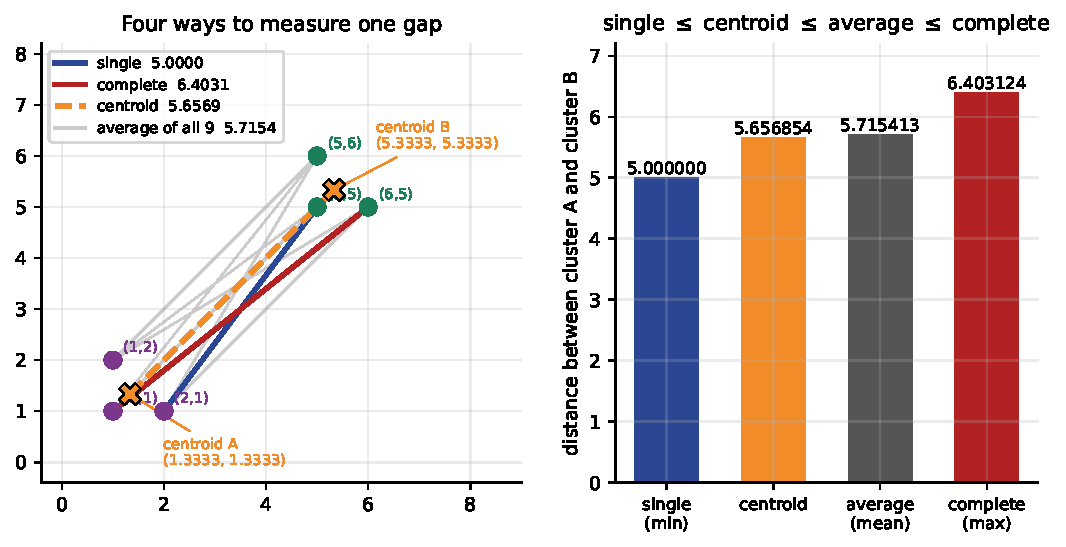
\includegraphics[width=0.84\textwidth]{linkage_distances.pdf}
  \caption{The four inter-cluster distances on two three-point clusters. The
    ordering single $\le$ centroid $\le$ average $\le$ complete holds here
    and the first and last always hold by definition.}
  \label{fig:linkfig}
\end{figure}

\begin{codeout}
ordering: single 5.0000 <= centroid 5.6569 <= average 5.7154 <= complete 6.4031
centroid <= average always: the distance between the means is at
most the mean of the distances (Jensen).  Gap here 0.058559.
\end{codeout}

Single is the minimum and complete the maximum of the same nine numbers, so
single $\le$ average $\le$ complete holds by definition. Centroid $\le$
average is Jensen's inequality: the distance between the means is at most the
mean of the distances, because the norm is convex. Here the gap is
$0.058559$, small because the two clusters are compact and far apart; on
elongated clusters it is large.

\subsection{Ward, which is not a distance at all}

The fifth linkage rule you will meet measures something different: how much
within-cluster scatter merging would \emph{create}.

\begin{equation}
  \Delta(A,B) = \mathrm{SSE}(A \cup B) - \mathrm{SSE}(A) - \mathrm{SSE}(B)
  = \frac{n_A n_B}{n_A + n_B}\,\|\bar{c}_A - \bar{c}_B\|^2.
  \label{eq:ward}
\end{equation}

\begin{codeout}
SSE(A) 1.333333 + SSE(B) 1.333333 = 2.666667
SSE(A union B)                = 50.666667
increase on merging           = 48.000000
closed form (nA nB/(nA+nB)) ||cA-cB||^2 = 48.000000   diff 1.42e-14
\end{codeout}

Check the closed form by hand: $n_A = n_B = 3$, so the coefficient is
$9/6 = 1.5$, and $\|\bar{c}_A - \bar{c}_B\|^2 = (4\sqrt2)^2 = 32$, giving
$1.5 \times 32 = 48$.

\begin{codeout}
single    height of the final merge  5.000000
complete  height of the final merge  6.403124
average   height of the final merge  5.715413
centroid  height of the final merge  5.656854
ward      height of the final merge  9.797959
\end{codeout}

\begin{caution}[Do not compare a Ward height with a linkage distance]
\texttt{scipy} reports the Ward merge at $9.797959$ where the other four
report numbers near $5.7$. It is measuring a different quantity in different
units --- \texttt{scipy} in fact reports $\sqrt{2\Delta}$ for Ward, so
$\sqrt{2 \times 48} = 9.797959$. A dendrogram's $y$-axis only means something
relative to its own linkage.
\end{caution}

% =========================================================================
\section{Does any of this actually change a clustering?}
\label{sec:realdata}

Every argument above has been about the input. Here is the output. One
algorithm, one dataset, one setting --- only the distance and the scaling
change.

\begin{lstlisting}
w = load_wine(); X, y = w.data, w.target
Xz = StandardScaler().fit_transform(X)
for m in ["euclidean", "manhattan", "chebyshev", "cosine"]:
    lab = AgglomerativeClustering(n_clusters=3, metric=m,
                                  linkage="average").fit_predict(X)
    print(m, adjusted_rand_score(y, lab))
\end{lstlisting}
\begin{codeout}
AgglomerativeClustering(n_clusters=3, linkage='average')
metric              ARI raw ARI z-scored
euclidean            0.2926      -0.0054
manhattan            0.3186       0.4730
chebyshev            0.2926      -0.0068
cosine               0.0535       0.7847
kmeans (L2sq)        0.3711       0.8975
\end{codeout}

\begin{figure}[htbp]
  \centering
  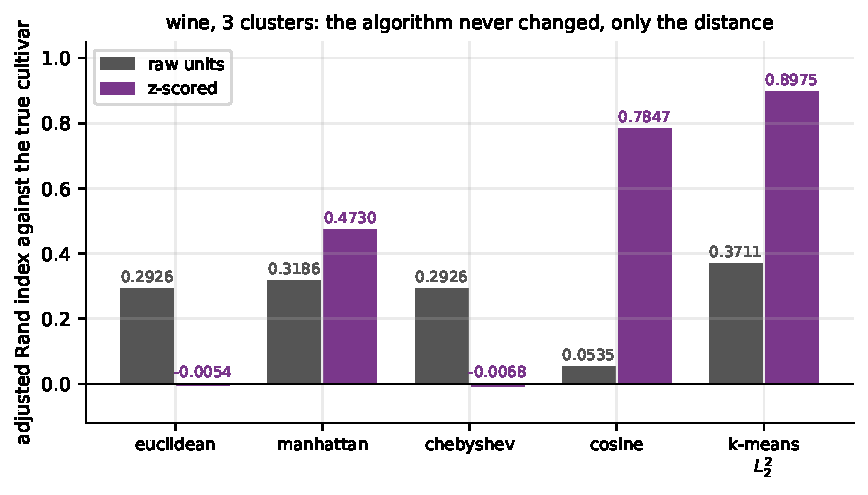
\includegraphics[width=0.74\textwidth]{wine_distance_choice.pdf}
  \caption{Ten runs on \texttt{wine} with three clusters, scored against the
    true cultivar by the adjusted Rand index. The spread from $-0.0068$ to
    $0.8975$ is entirely the distance and the scaling.}
  \label{fig:winefig}
\end{figure}

The adjusted Rand index scores agreement with the true cultivar labels; $0$
is chance and $1$ is perfect. The range across that table is $0.0535$ to
$0.8975$, and \emph{nothing about the algorithm changed between any two
rows}.

Two results in it need honest handling rather than a headline.

\textbf{Standardising made one row worse.} Average-linkage Euclidean fell
from $0.2926$ to $-0.0054$, which is worse than chance. Look at what it
produced:

\begin{codeout}
  raw       cluster sizes [130, 42, 6]
  z-scored  cluster sizes [174, 1, 3]
\end{codeout}

That is not a distance failure. It is average linkage peeling off two tiny
groups of outliers, which became visible once standardising let the
small-scale columns speak. The lesson is not ``do not standardise'' --- the
$k$-means row went from $0.3711$ to $0.8975$ on the same transformation ---
but \textbf{choose the distance and the linkage together}, which is precisely
what the next lecture is about.

\textbf{Cosine on raw \texttt{wine} did badly, correctly.} Cosine discards
vector length. On raw \texttt{wine}, length is almost entirely proline
(Section~\ref{sec:standard}: $0.997738$ of the raw squared distance), and
proline separates the cultivars --- so throwing the length away throws the
signal away. On text, where length is document length, throwing it away is
exactly right. And the bridge of Section~\ref{sec:cosine} holds on real data:

\begin{codeout}
after L2-normalising the rows, Euclidean and cosine agree:
  ARI(euclidean on normalised rows) = 0.0535
  ARI(cosine on raw rows)           = 0.0535
  identical partitions: True
\end{codeout}

\begin{keyidea}[The distance is a modelling decision]
Not a detail, not a default, not a hyperparameter to grid-search after the
fact. It encodes what you believe ``similar'' means for these objects, and no
amount of algorithm choice will recover a badly chosen one.
\end{keyidea}

% =========================================================================
\section{Summary}
\label{sec:summary}

\begin{enumerate}[leftmargin=*]
  \item A \textbf{similarity} is large for alike objects, a
    \textbf{dissimilarity} small. Clustering algorithms consume the
    $n\times n$ dissimilarity matrix, not the data, and it costs
    $n(n-1)/2$ numbers --- $40$ GB at $n = 100\,000$.
  \item A dissimilarity is a \textbf{metric} if it satisfies non-negativity,
    identity of indiscernibles, symmetry and the triangle inequality.
    \textbf{Squared Euclidean} distance and \textbf{cosine distance} violate
    the triangle inequality; \textbf{KL divergence} violates symmetry.
  \item The \textbf{Minkowski} family $d_p = (\sum_f|x_f-y_f|^p)^{1/p}$
    covers Manhattan ($p{=}1$), Euclidean ($p{=}2$) and Chebyshev
    ($p{\to}\infty$). On $(1,2)$ and $(4,6)$: $7$, $5$, $4.497941$ at
    $p=3$, and $4$.
  \item $d_1 \ge d_2 \ge \cdots \ge d_\infty$ always. $p$ controls how
    heavily one badly disagreeing attribute is punished; on $q=(0,0)$ with
    $u=(3,3)$ and $v=(4.5,0)$, $p=1$ picks $v$ and every $p \ge 2$ picks $u$.
  \item \textbf{Cosine} measures direction and discards length. $A=(1,2)$,
    $B=10A$, $C=(2,1)$: Euclidean says $C$ ($1.414214$ against $20.124612$),
    cosine says $B$ ($1.0000$ against $0.8000$).
  \item $\|\hat a - \hat b\|^2 = 2(1-\cos)$, so cosine \emph{is} Euclidean
    distance on $L_2$-normalised rows, and $\sqrt{2(1-\cos)}$ is a metric
    where $1-\cos$ is not.
  \item \textbf{Binary}: build $q, r, s, t$. \textbf{Simple matching}
    $(q+t)/p$ for symmetric attributes, \textbf{Jaccard} $q/(q+r+s)$ for
    asymmetric. The entire distinction is whether a shared \emph{absence} is
    evidence.
  \item The two can rank the same two pairs in \textbf{opposite orders}
    ($0.8000$ vs $0.6000$ against $0.3333$ vs $0.6000$), and padding with
    shared zeros drives simple matching to $0.9980$ while Jaccard stays at
    $0.3333$.
  \item \textbf{Nominal}: the mismatch ratio $(p-m)/p$. One-hot with $L_1$
    reproduces it exactly; with $L_2$ the ranking survives but the gaps
    compress by a square root; with \emph{standardised} dummies the ranking
    can reverse, because a rare level acquires a large weight.
  \item \textbf{Ordinal}: $z = (r-1)/(M-1)$, then treat as numeric. Dividing
    by $M-1$ makes scales of different length commensurable. Equal spacing is
    an assumption.
  \item \textbf{Mixed}: Gower, $\sum_f \delta_f d_f / \sum_f \delta_f$. A
    $0$--$0$ pair on an asymmetric binary attribute sets $\delta_f = 0$ and
    leaves \emph{both} sums. $d(A,B) = 0.340686$ over six attributes,
    $d(B,D) = 0.372794$ over five.
  \item \textbf{Standardisation changes which object is nearest} ---
    $94.4\%$ of \texttt{wine} rows. Mean-absolute-deviation scaling is the
    robust alternative; $\sigma/s \to \sqrt{\pi/2} = 1.2533$ for a Gaussian
    column, and only rises above that when the tail is real.
  \item \textbf{Centroid} is the mean and usually not a data point;
    \textbf{medoid} is a data point and needs only the dissimilarity matrix.
    That difference is $k$-means against $k$-medoids.
  \item Inter-cluster distances on the worked pair: single $5.000000$,
    centroid $5.656854$, average $5.715413$, complete $6.403124$, in that
    order. Ward measures the SSE increase, $48.000000$, and is not
    comparable with the other four.
  \item On \texttt{wine} the same algorithm scored between $0.0535$ and
    $0.8975$ depending only on the distance and the scaling.
\end{enumerate}

% =========================================================================
\section{Practice questions}
\label{sec:practice}

Full worked solutions follow in Section~\ref{sec:solutions}. Questions 1, 3,
4, 5 and 6 are pure hand computation --- do them with a pen before you look.

\begin{enumerate}[leftmargin=*]
  \item \textbf{(Minkowski, by hand.)} For $x = (2, 7, 3)$ and
    $y = (6, 4, 3)$, compute $d_1$, $d_2$, $d_3$ and $d_\infty$ to six
    decimal places. Then state, without computing, whether $d_{10}$ is
    larger or smaller than $d_3$, and why.

  \item \textbf{(Axioms.)} Show that $d(x,y) = \|x-y\|^2$ fails the triangle
    inequality by giving a counter-example with three points in
    $\mathbb{R}^1$, and state which \emph{other} three axioms it does
    satisfy. Then say why $k$-means using this measure is not a defect.

  \item \textbf{(Cosine, by hand.)} Two customers' monthly spend on three
    categories, in rupees: $P = (200, 400, 400)$ and
    $Q = (1000, 2000, 2000)$; a third, $R = (400, 400, 200)$. Compute the
    Euclidean distance and the cosine similarity for all three pairs. Which
    customer is $P$'s nearest neighbour under each measure? Which measure
    would you use to find customers with the same \emph{spending pattern}
    regardless of budget, and why?

  \item \textbf{(Binary, by hand.)} Four students, five asymmetric binary
    attributes recording whether they have used a tool:
    \begin{center}
    \begin{tabular}{lccccc}
      \toprule
      & git & docker & latex & pandas & spark \\ \midrule
      W & 1 & 0 & 1 & 1 & 0 \\
      X & 1 & 1 & 0 & 1 & 0 \\
      Y & 1 & 0 & 1 & 1 & 1 \\
      Z & 0 & 0 & 0 & 0 & 0 \\ \bottomrule
    \end{tabular}
    \end{center}
    Build the $q,r,s,t$ table for all six pairs. Compute both the simple
    matching and the Jaccard coefficient for each. Which pair does each
    coefficient call the most similar, and what does student $Z$ reveal
    about the difference?

  \item \textbf{(Nominal and ordinal, by hand.)} Three job applications with
    two nominal attributes (\texttt{stream} $\in$ \{CSE, ECE\},
    \texttt{city} $\in$ \{Delhi, Pune, Delhi\}) and one ordinal attribute
    (\texttt{grade} $\in$ \{third, second, first, distinction\}):
    \begin{center}
    \begin{tabular}{llll}
      \toprule
      & stream & city & grade \\ \midrule
      U & CSE & Delhi & distinction \\
      V & CSE & Pune  & second \\
      W & ECE & Delhi & first \\ \bottomrule
    \end{tabular}
    \end{center}
    Compute the nominal mismatch ratio for each pair. Map the ordinal
    attribute with \eqref{eq:ordinal} and give $|z_i - z_j|$ for each pair.
    Then compute the unweighted mean of the three per-attribute
    dissimilarities for each pair and rank them.

  \item \textbf{(Gower, by hand.)} Using the applicant table of
    Section~\ref{sec:mixed}, compute $d(C,D)$ showing every $\delta_f$ and
    every $d_f$. State the denominator and justify it.

  \item \textbf{(Standardisation.)} A dataset has two columns: \texttt{income}
    with standard deviation $30\,000$ and \texttt{age} with standard
    deviation $12$. Two candidate neighbours of a query differ from it by
    $(\Delta\texttt{income}, \Delta\texttt{age}) = (1500, 20)$ and
    $(4000, 2)$. Which is nearer in raw units and which after z-scoring?
    Give both distances in both scalings.

  \item \textbf{(z-score against MAD.)} For $x = 5, 6, 7, 8, 9, 60$ compute
    the mean, the population standard deviation and the mean absolute
    deviation, then the ratio $\sigma/s$. Compare it with $\sqrt{\pi/2}$ and
    say what the comparison tells you.

  \item \textbf{(Cluster distances, by hand.)} $A = \{(0,0), (2,0)\}$ and
    $B = \{(5,1), (7,3), (6,0)\}$. Compute all six cross distances, then the
    single, complete, average and centroid distances between $A$ and $B$.
    Verify the ordering claim of Section~\ref{sec:centroid} and, if it fails
    anywhere, say which inequality is not guaranteed.

  \item \textbf{(Judgement.)} You are clustering hospital records. The
    columns are: \texttt{age} (years), \texttt{ward} (one of eight),
    \texttt{triage\_level} (one of five, ordered), \texttt{is\_male},
    \texttt{tested\_positive\_for\_MRSA}, and forty
    \texttt{prescribed\_drug\_X} flags of which each patient has three or
    four set. Specify the complete distance you would use: the treatment of
    every column type, the symmetric/asymmetric decision for every binary
    column, the scaling, and the combination rule. Then name one thing that
    would go wrong if you instead z-scored the whole table after
    label-encoding.
\end{enumerate}

% =========================================================================
\section{Solutions}
\label{sec:solutions}

\paragraph{1. Minkowski by hand.}
The componentwise gaps are $|2-6| = 4$, $|7-4| = 3$, $|3-3| = 0$.
\begin{align*}
  d_1 &= 4 + 3 + 0 = 7.000000 \\
  d_2 &= \sqrt{16 + 9 + 0} = \sqrt{25} = 5.000000 \\
  d_3 &= (64 + 27 + 0)^{1/3} = 91^{1/3} = 4.497941 \\
  d_\infty &= \max(4,3,0) = 4.000000
\end{align*}
(These are the same four numbers as the worked example in
Section~\ref{sec:minkowski}, because the multiset of gaps is the same
$\{3,4\}$ plus a zero, and a zero gap contributes nothing at any $p$.)
$d_{10} < d_3$: by \eqref{eq:order} the sequence is non-increasing in $p$,
converging down to $d_\infty = 4$. Explicitly $d_{10} = 4.021974$.

\paragraph{2. Axioms.}
Take $a = 0$, $b = 1$, $c = 2$ on the line. Then $d(a,b) = 1$,
$d(b,c) = 1$, $d(a,c) = 4$, and $4 > 1 + 1$, so \eqref{eq:ax4} fails.
It \emph{does} satisfy the other three: $\|x-y\|^2 \ge 0$ always;
$\|x-y\|^2 = 0$ if and only if $x = y$; and $\|x-y\|^2 = \|y-x\|^2$.

$k$-means is not defective, because it never uses the triangle inequality to
justify its answer --- it uses squared Euclidean distance as an
\emph{objective function}, and the identity \eqref{eq:sseident} shows the
mean is exactly the minimiser of that objective. What you lose is the ability
to use triangle-inequality pruning naively, and the right to describe the
number $k$-means minimises as a distance. Note also that squaring is monotone,
so the nearest centroid under squared Euclidean is the nearest centroid under
Euclidean: the assignment step is unaffected.

\paragraph{3. Cosine by hand.}
$Q = 5P$, so they point in the same direction.
\begin{align*}
  \|P\| &= \sqrt{200^2 + 400^2 + 400^2} = \sqrt{40000 + 160000 + 160000}
    = \sqrt{360000} = 600 \\
  \|Q\| &= 5 \times 600 = 3000 \\
  \|R\| &= \sqrt{160000 + 160000 + 40000} = \sqrt{360000} = 600
\end{align*}
Euclidean distances:
\begin{align*}
  d(P,Q) &= \sqrt{800^2 + 1600^2 + 1600^2} = 4 \times 600 = 2400.000000 \\
  d(P,R) &= \sqrt{200^2 + 0^2 + 200^2} = \sqrt{80000} = 282.842712 \\
  d(Q,R) &= \sqrt{600^2 + 1600^2 + 1800^2} = \sqrt{360000+2560000+3240000}
    = \sqrt{6160000} = 2481.934729
\end{align*}
Cosine similarities:
\begin{align*}
  \cos(P,Q) &= \frac{5\|P\|^2}{\|P\| \cdot 5\|P\|} = 1.000000 \\
  \cos(P,R) &= \frac{200{\cdot}400 + 400{\cdot}400 + 400{\cdot}200}
    {600 \times 600} = \frac{80000+160000+80000}{360000}
    = \frac{320000}{360000} = 0.888889 \\
  \cos(Q,R) &= \cos(P,R) = 0.888889 \quad
    \text{(cosine is invariant to scaling either vector)}
\end{align*}
Under Euclidean distance $P$'s nearest neighbour is $R$ ($282.84$ against
$2400$); under cosine it is $Q$ ($1.0000$ against $0.888889$). To find
customers with the same spending \emph{pattern} regardless of budget, use
cosine: $Q$ spends five times as much as $P$ on every category, so $Q$ has
exactly $P$'s pattern, and Euclidean distance is measuring the budget
difference rather than the pattern difference.

\paragraph{4. Binary by hand.}
Count, for each pair, the four buckets over the five attributes.
\begin{center}
\begin{tabular}{lcccccc}
  \toprule
  pair & $q$ & $r$ & $s$ & $t$ & SMC $=(q{+}t)/5$ & $J = q/(q{+}r{+}s)$ \\
  \midrule
  W,X & 2 & 1 & 1 & 1 & $3/5 = 0.6000$ & $2/4 = 0.5000$ \\
  W,Y & 3 & 0 & 1 & 1 & $4/5 = 0.8000$ & $3/4 = 0.7500$ \\
  W,Z & 0 & 3 & 0 & 2 & $2/5 = 0.4000$ & $0/3 = 0.0000$ \\
  X,Y & 2 & 1 & 2 & 0 & $2/5 = 0.4000$ & $2/5 = 0.4000$ \\
  X,Z & 0 & 3 & 0 & 2 & $2/5 = 0.4000$ & $0/3 = 0.0000$ \\
  Y,Z & 0 & 4 & 0 & 1 & $1/5 = 0.2000$ & $0/4 = 0.0000$ \\
  \bottomrule
\end{tabular}
\end{center}
Both coefficients call $W,Y$ the most similar pair, at $0.8000$ and
$0.7500$. The interesting rows are the ones involving $Z$, who has used
nothing. Simple matching gives $W,Z$ and $X,Z$ a score of $0.4000$ ---
\emph{the same as $X,Y$}, a pair who share two tools. Jaccard gives them
$0.0000$, which is right: $Z$ has nothing in common with anybody, and the
only thing $Z$ shares with $W$ is the failure to use Docker and Spark.
Because these attributes are asymmetric, Jaccard is the correct choice and
simple matching would place $Z$ in the middle of the cohort rather than at
its edge.

\paragraph{5. Nominal and ordinal by hand.}
Nominal mismatch ratio over the two nominal attributes ($p = 2$):
\begin{center}
\begin{tabular}{lcccc}
  \toprule
  pair & stream & city & $m$ & $(2-m)/2$ \\ \midrule
  U,V & same (CSE) & differ & 1 & $0.500000$ \\
  U,W & differ & same (Delhi) & 1 & $0.500000$ \\
  V,W & differ & differ & 0 & $1.000000$ \\
  \bottomrule
\end{tabular}
\end{center}
Ordinal with $M = 4$: third $\to 0$, second $\to 1/3 = 0.333333$,
first $\to 2/3 = 0.666667$, distinction $\to 1$. So $U = 1.000000$,
$V = 0.333333$, $W = 0.666667$, and
\[
  |z_U - z_V| = 0.666667, \qquad
  |z_U - z_W| = 0.333333, \qquad
  |z_V - z_W| = 0.333333.
\]
Unweighted mean of the three per-attribute dissimilarities (stream, city,
grade):
\begin{align*}
  d(U,V) &= \tfrac{1}{3}(0 + 1 + 0.666667) = 0.555556 \\
  d(U,W) &= \tfrac{1}{3}(1 + 0 + 0.333333) = 0.444444 \\
  d(V,W) &= \tfrac{1}{3}(1 + 1 + 0.333333) = 0.777778
\end{align*}
Ranking, closest first: $U,W$ $(0.444444)$, then $U,V$ $(0.555556)$, then
$V,W$ $(0.777778)$. Note that $U$ and $V$ tie with $U$ and $W$ on the nominal
part; the ordinal attribute breaks the tie.

\paragraph{6. Gower by hand.}
$C = (41, 18, \text{PhD}, \text{Mumbai}, 1, 0, 1)$ and
$D = (26, 3, \text{BTech}, \text{Delhi}, 0, 1, 0)$, with $R_{\text{age}} = 17$
and $R_{\text{exp}} = 16$.
\begin{center}
\begin{tabular}{lrrr}
  \toprule
  attribute $f$ & $\delta_f$ & $d_f$ & $\delta_f d_f$ \\ \midrule
  age & 1 & $|41-26|/17 = 15/17 = 0.882353$ & 0.882353 \\
  experience & 1 & $|18-3|/16 = 15/16 = 0.937500$ & 0.937500 \\
  degree & 1 & $|1.0 - 0.0| = 1.000000$ & 1.000000 \\
  city & 1 & Mumbai vs Delhi, $1.000000$ & 1.000000 \\
  car & 1 & $1$ vs $0$, $1.000000$ & 1.000000 \\
  python & 1 & $0$ vs $1$, $1.000000$ & 1.000000 \\
  patent & 1 & $1$ vs $0$, $1.000000$ & 1.000000 \\
  \midrule
  SUM & \textbf{7} & & \textbf{6.819853} \\
  \bottomrule
\end{tabular}
\end{center}
\[
  d(C,D) = \frac{6.819853}{7} = 0.974265
\]
The denominator is $7$: \emph{no} attribute is skipped, because on each of
the three asymmetric binary attributes at least one of the two objects is
$1$. $C$ and $D$ are the most dissimilar pair in the table, which is what the
matrix in Section~\ref{sec:mixed} reports.

\paragraph{7. Standardisation.}
Raw:
\[
  d_1 = \sqrt{1500^2 + 20^2} = \sqrt{2\,250\,000 + 400} = 1500.133327,
  \qquad
  d_2 = \sqrt{4000^2 + 2^2} = 4000.000500
\]
so the first candidate is nearer, and the age column contributed
$0.000133$ to the answer --- the income column carries $0.999822$ of
candidate 1's squared distance and $1.000000$ of candidate 2's.

After z-scoring, divide each gap by its column's standard deviation:
\[
  d_1 = \sqrt{(1500/30000)^2 + (20/12)^2} = \sqrt{0.05^2 + 1.666667^2}
      = \sqrt{0.0025 + 2.777778} = 1.667416
\]
\[
  d_2 = \sqrt{(4000/30000)^2 + (2/12)^2} = \sqrt{0.133333^2 + 0.166667^2}
      = \sqrt{0.017778 + 0.027778} = 0.213437
\]
so the \emph{second} candidate is nearer, by a factor of nearly eight. The
neighbour changed identity, exactly as in Section~\ref{sec:standard}. The
mechanism is the same: in raw units ``distance'' meant ``income
difference'', and the age column --- which after scaling is the column that
decides the answer --- was not consulted.

\paragraph{8. z-score against MAD.}
$n = 6$, sum $= 5+6+7+8+9+60 = 95$, so $\mu = 95/6 = 15.833333$.
Deviations: $-10.833333, -9.833333, -8.833333, -7.833333, -6.833333,
+44.166667$.
\[
  \sigma = \sqrt{\frac{117.361 + 96.694 + 78.028 + 61.361 + 46.694
    + 1950.694}{6}} = \sqrt{\frac{2350.833}{6}} = \sqrt{391.805556}
    = 19.794079
\]
\[
  s = \frac{10.833333+9.833333+8.833333+7.833333+6.833333+44.166667}{6}
    = \frac{88.333333}{6} = 14.722222
\]
\[
  \sigma / s = 19.794079 / 14.722222 = 1.344503
\]
Against $\sqrt{\pi/2} = 1.253314$, the ratio is $7.28\%$ higher, which says
this column has a heavier tail than a Gaussian --- unsurprising, since one
value in six is an outlier. The gap between two neighbouring ordinary values
is $1/\sigma = 0.050520$ under z-scoring and $1/s = 0.067925$ under MAD
scaling, so MAD keeps them $34.5\%$ further apart.

\paragraph{9. Cluster distances by hand.}
$A = \{a_1 = (0,0),\, a_2 = (2,0)\}$, $B = \{b_1 = (5,1),\, b_2 = (7,3),\,
b_3 = (6,0)\}$.
\begin{align*}
  d(a_1,b_1) &= \sqrt{25+1} = \sqrt{26} = 5.099020 &
  d(a_2,b_1) &= \sqrt{9+1} = \sqrt{10} = 3.162278 \\
  d(a_1,b_2) &= \sqrt{49+9} = \sqrt{58} = 7.615773 &
  d(a_2,b_2) &= \sqrt{25+9} = \sqrt{34} = 5.830952 \\
  d(a_1,b_3) &= \sqrt{36+0} = 6.000000 &
  d(a_2,b_3) &= \sqrt{16+0} = 4.000000
\end{align*}
\begin{align*}
  d_{\text{single}} &= 3.162278 \quad (a_2 b_1) \\
  d_{\text{complete}} &= 7.615773 \quad (a_1 b_2) \\
  d_{\text{average}} &= \frac{5.099020 + 7.615773 + 6.000000
    + 3.162278 + 5.830952 + 4.000000}{6} = \frac{31.708022}{6} = 5.284670
\end{align*}
Centroids: $\bar{c}_A = (1, 0)$ and
$\bar{c}_B = \big(\frac{5+7+6}{3}, \frac{1+3+0}{3}\big) = (6, 4/3)$, so
\[
  d_{\text{centroid}} = \sqrt{5^2 + (4/3)^2} = \sqrt{25 + 1.777778}
    = \sqrt{26.777778} = 5.174725
\]
Ordering: single $3.162278 \le$ centroid $5.174725 \le$ average $5.284670
\le$ complete $7.615773$. Single $\le$ average $\le$ complete is guaranteed
(they are the minimum, mean and maximum of the same six numbers) and
centroid $\le$ average is guaranteed by Jensen's inequality. What is
\textbf{not} guaranteed is single $\le$ centroid. Counter-example:
$A = \{(-3,0),(3,0)\}$ and $B = \{(0,-3),(0,3)\}$ have the \emph{same}
centroid $(0,0)$, so $d_{\text{centroid}} = 0.000000$, while all four cross
distances equal $\sqrt{9+9} = 4.242641$, so
$d_{\text{single}} = 4.242641 > 0$. The two relations that always hold are
single $\le$ average $\le$ complete and centroid $\le$ average.

\paragraph{10. Judgement.}
A defensible specification:

\begin{itemize}[leftmargin=*]
  \item \texttt{age}: numeric. Range-normalise (Gower) or z-score, and state
    which. A range normalisation is safer here because hospital ages have a
    hard floor at zero and a soft ceiling, so the range is meaningful.
  \item \texttt{ward}: nominal with eight levels. Mismatch contribution
    $0$ or $1$. \textbf{Do not label-encode.} If you have domain knowledge
    that some wards are clinically adjacent, that is an argument for a
    custom per-pair table, not for an alphabetical integer.
  \item \texttt{triage\_level}: ordinal with $M = 5$. Map with
    $(r-1)/4$ and use $|z_i - z_j|$. Record the equal-spacing assumption;
    triage scales are usually \emph{not} equally spaced, so this is a place
    to consider a custom mapping.
  \item \texttt{is\_male}: \textbf{symmetric} binary. Two men are as alike as
    two women; contribution $0$ or $1$ with $\delta_f = 1$ always.
  \item \texttt{tested\_positive\_for\_MRSA}: \textbf{asymmetric}. A shared
    positive is highly informative, a shared negative is the default state of
    almost every patient. $\delta_f = 0$ when both are negative.
  \item The forty \texttt{prescribed\_drug\_X} flags: \textbf{asymmetric},
    and sparse --- three or four set out of forty. These are exactly the
    market-basket case of Section~\ref{sec:swamp}. Treat them as a Jaccard
    block, or equivalently give each of the forty $\delta_f = 0$ when both
    patients are $0$.
  \item \textbf{Combination}: Gower, equation~\eqref{eq:gower} --- with one
    weighting problem you must address explicitly. Forty drug flags against
    five other columns will dominate the average even under Jaccard
    treatment. Either down-weight the block, or compute a single Jaccard
    dissimilarity over the forty and enter that as one attribute. Say which
    you did.
\end{itemize}

If instead you z-scored the whole table after label-encoding, three things go
wrong, any one of which invalidates the result. \texttt{ward} acquires an
order and a spacing from the alphabet, so ``Cardiology'' and ``Casualty''
become nearby by accident of spelling. The thirty-seven zero entries in each
patient's drug row become evidence of similarity --- the shared-absence
problem of Section~\ref{sec:swamp} --- so every patient starts to look like
every other. And z-scoring the sparse flags divides each by
$\sqrt{\pi_f(1-\pi_f)}$, so the \emph{rarest} drugs get the largest weights
and the clustering ends up driven by which two patients happen to share one
unusual prescription.

% =========================================================================
\section{References and further reading}
\label{sec:refs}

All links were checked on 24 August 2026. Free resources are marked
\textbf{[free]}.

\subsection*{Textbooks}

\begin{itemize}[leftmargin=*]
  \item Han, Kamber and Pei, \emph{Data Mining: Concepts and Techniques},
    3rd edition, Morgan Kaufmann, 2012. \textbf{The prescribed text for this
    lecture, and it is the source of the notation used throughout.} \S2.4
    ``Measuring Data Similarity and Dissimilarity'' is this entire lecture:
    \S2.4.1 the data matrix and the dissimilarity matrix
    (Section~\ref{sec:vocab}); \S2.4.2 nominal attributes and the
    $(p-m)/p$ formula (Section~\ref{sec:nominal}); \S2.4.3 binary
    attributes, the contingency table, the simple matching and Jaccard
    coefficients and the Jack/Jim/Mary example used in
    Section~\ref{sec:binary}; \S2.4.4 numeric attributes, Minkowski,
    Manhattan, Euclidean and supremum distance, with the
    mean-absolute-deviation standardisation of
    equation~\eqref{eq:mad}; \S2.4.5 ordinal attributes and
    $(r-1)/(M-1)$; \S2.4.6 mixed types and the Gower-style formula
    \eqref{eq:gower}; \S2.4.7 cosine similarity. \S10.2 gives the centroid,
    medoid and the four inter-cluster distances of
    Section~\ref{sec:centroid}.
  \item Tan, Steinbach, Karpatne and Kumar, \emph{Introduction to Data
    Mining}, 2nd edition, Pearson, 2019. Chapter 2 \S2.4 is a second and
    unusually careful treatment of proximity measures, including the
    symmetric/asymmetric distinction, the simple matching versus Jaccard
    comparison, and a longer list of binary coefficients than the prescribed
    text gives.
  \item James, Witten, Hastie, Tibshirani and Taylor, \emph{An Introduction
    to Statistical Learning with Python}. \textbf{[free]} \S12.4 clustering;
    \S12.4.2's discussion of correlation-based distance against Euclidean
    distance for the online-shopper example is the same argument as
    Section~\ref{sec:cosine}, and \S12.4.3 (``Practical Issues in
    Clustering'') is Section~\ref{sec:standard} in different words.
    \url{https://www.statlearning.com/}
  \item Hastie, Tibshirani and Friedman, \emph{The Elements of Statistical
    Learning}, 2e, Springer. \textbf{[free]} \S14.3.1--14.3.3 are the formal
    treatment: proximity matrices, dissimilarities based on attributes, and
    ``Object Dissimilarity'', where \S14.3.3 makes precisely the point of
    Section~\ref{sec:standard} --- that standardising every attribute to
    unit variance is \emph{not} automatically the right thing to do, because
    it can suppress the very attribute that separates the clusters.
    \url{https://hastie.su.domains/ElemStatLearn/}
  \item M\"uller and Guido, \emph{Introduction to Machine Learning with
    Python}, O'Reilly, 2016. \S3.3 preprocessing and scaling, which is the
    library-facing version of Section~\ref{sec:standard}, and \S3.5 on
    clustering. Notebooks \textbf{[free]}:
    \url{https://github.com/amueller/introduction_to_ml_with_python}
  \item Murphy, \emph{Probabilistic Machine Learning: An Introduction}, MIT
    Press, 2022. \textbf{[free]} Chapter 6 covers information-theoretic
    quantities including the KL divergence of Section~\ref{sec:violators}
    and why it is not symmetric.
    \url{https://probml.github.io/pml-book/book1.html}
\end{itemize}

\subsection*{Online courses}

\begin{sloppypar}
\begin{itemize}[leftmargin=*]
  \item \textbf{NPTEL, Data Mining} --- Prof.\ Pabitra Mitra, IIT Kharagpur.
    The closest match to this lecture of any course on the portal: it follows
    the Han--Kamber--Pei chapter structure, so its data-preprocessing and
    clustering weeks map onto \S2.4 and \S10.2 directly. \textbf{[free]}
    \url{https://nptel.ac.in/courses/106105174}
  \item \textbf{NPTEL, Introduction to Machine Learning} --- Prof.\ Balaraman
    Ravindran, IIT Madras; the reference course for the semester. The
    clustering week develops the distance measures before the algorithms, in
    the same order as these notes. \textbf{[free]}
    \url{https://nptel.ac.in/courses/106106139}
  \item \textbf{NPTEL, Introduction to Machine Learning --- IITKGP} ---
    Prof.\ Sudeshna Sarkar, IIT Kharagpur. A second treatment worked at the
    board, if the first does not land. \textbf{[free]}
    \url{https://nptel.ac.in/courses/106105152}
  \item \textbf{SWAYAM} --- the national portal hosting NPTEL, with
    certification cycles. \textbf{[free]} \url{https://swayam.gov.in/}
  \item \textbf{Google, Clustering} --- a short course (about 110 minutes)
    with a module called ``Manual similarity measure'' that works through
    combining numeric, categorical and ordinal columns into one similarity,
    exactly as Section~\ref{sec:mixed} does. \textbf{[free]}
    \url{https://developers.google.com/machine-learning/clustering}
\end{itemize}
\end{sloppypar}

\subsection*{Videos}

\begin{itemize}[leftmargin=*]
  \item StatQuest with Josh Starmer, \emph{Cosine Similarity, Clearly
    Explained!!!} --- the geometry of Section~\ref{sec:cosine} at a
    whiteboard, including why it is used for text and how it relates to
    correlation. Watch this one first. \textbf{[free]}
    \url{https://youtu.be/e9U0QAFbfLI}
  \item Mahesh Huddar, \emph{How to find Euclidean Manhattan Minkowski
    distance Supremum distance Cosine Similarity} --- a single solved
    numerical example covering all four Minkowski cases plus cosine, in the
    examination format. \textbf{[free]}
    \url{https://youtu.be/gwtTM9M6ugU}
  \item Mahesh Huddar, \emph{Simple Matching Coefficient SMC Jaccard
    Coefficient \& Hamming Distance Solved Example} --- the contingency table
    of Section~\ref{sec:binary} worked on a different table, with the
    symmetric/asymmetric decision made explicitly. \textbf{[free]}
    \url{https://youtu.be/R0ORgpi25d0}
  \item Binod Suman Academy, \emph{Proximity Measures - 7 $|$ Mixed Attribute
    $|$ Data Mining} --- the Gower calculation of Section~\ref{sec:mixed}
    worked step by step. It is the last of a numbered series whose earlier
    parts map onto these notes almost section by section: part 2 nominal,
    parts 3--4 binary, part 5 ordinal, part 6 numeric. \textbf{[free]}
    \url{https://youtu.be/aVUMDYPXLxM}
\end{itemize}

\subsection*{Documentation and interactive explainers}

\begin{itemize}[leftmargin=*]
  \item \texttt{scipy.spatial.distance} --- the reference for every measure
    in these notes. The module docstring lists all of
    \texttt{euclidean}, \texttt{cityblock}, \texttt{minkowski},
    \texttt{chebyshev}, \texttt{cosine}, \texttt{jaccard} and
    \texttt{hamming} with their exact definitions, which is the place to
    check whether a function returns a similarity or a dissimilarity.
    \textbf{[free]}
    \url{https://docs.scipy.org/doc/scipy/reference/spatial.distance.html}
  \item \texttt{scipy.spatial.distance.pdist} --- the condensed
    distance-matrix function of Section~\ref{sec:vocab}, with the full metric
    list and the storage convention. \textbf{[free]}
    \url{https://docs.scipy.org/doc/scipy/reference/generated/scipy.spatial.distance.pdist.html}
  \item \texttt{scipy.cluster.hierarchy.linkage} --- the linkage formulas of
    Section~\ref{sec:centroid} written out, including the fact that the Ward
    height is $\sqrt{2\Delta}$ rather than $\Delta$. \textbf{[free]}
    \url{https://docs.scipy.org/doc/scipy/reference/generated/scipy.cluster.hierarchy.linkage.html}
  \item scikit-learn user guide, \emph{Pairwise metrics, Affinities and
    Kernels} --- states the metric axioms in the documentation's own words
    and gives the cosine-similarity section that
    equation~\eqref{eq:bridge} formalises. \textbf{[free]}
    \url{https://scikit-learn.org/stable/modules/metrics.html}
  \item scikit-learn user guide, \emph{Clustering} --- \S2.3.6 covers
    \texttt{AgglomerativeClustering} and the \texttt{metric} and
    \texttt{linkage} arguments used in Section~\ref{sec:realdata}.
    \textbf{[free]}
    \url{https://scikit-learn.org/stable/modules/clustering.html}
  \item scikit-learn example, \emph{Compare the effect of different scalers
    on data with outliers} --- Section~\ref{sec:standard} made visual, with
    \texttt{StandardScaler}, \texttt{RobustScaler} and five others on the
    same heavy-tailed data. \textbf{[free]}
    \url{https://scikit-learn.org/stable/auto_examples/preprocessing/plot_all_scaling.html}
\end{itemize}

\subsection*{Articles}

\begin{itemize}[leftmargin=*]
  \item J.\ C.\ Gower, ``A General Coefficient of Similarity and Some of Its
    Properties'', \emph{Biometrics} \textbf{27}(4), 857--871, 1971. The
    original paper behind equation~\eqref{eq:gower}. \S2 defines the
    $\delta_f$ indicator and \S3 proves that the resulting matrix is positive
    semi-definite, which is what makes it safe to feed to methods that assume
    a Euclidean embedding. \url{https://doi.org/10.2307/2528823}
  \item A.\ H.\ Lipkus, ``A proof of the triangle inequality for the Tanimoto
    distance'', \emph{Journal of Mathematical Chemistry} \textbf{26},
    263--265, 1999. Three pages, and they prove that the Jaccard
    \emph{distance} $1 - J$ is a metric --- the ``yes'' in the Jaccard row
    of the axiom table in Section~\ref{sec:axioms}, which is not obvious and
    is often asserted without evidence. The paper calls the coefficient by
    its other name, Tanimoto. \url{https://doi.org/10.1023/A:1019154432472}
  \item L.\ Hubert and P.\ Arabie, ``Comparing partitions'',
    \emph{Journal of Classification} \textbf{2}, 193--218, 1985. The adjusted
    Rand index used to score every clustering in
    Section~\ref{sec:realdata}, and the reason a value can be negative.
    \url{https://doi.org/10.1007/BF01908075}
\end{itemize}

\notesources{\AMLUnitVIISources}

\end{document}
